%
% Template Laporan Skripsi/Thesis Universitas Indonesia
%
% @author  Ichlasul Affan, Azhar Kurnia
% @version 2.1.0
%
% Dokumen ini dibuat berdasarkan standar IEEE dalam membuat class untuk
% LaTeX dan konfigurasi LaTeX yang digunakan Fahrurrozi Rahman ketika
% membuat laporan skripsi, yang kemudian diadaptasi oleh Andreas Febrian dan
% Lia Sadita untuk template skripsi tahun 2010.
% Konfigurasi template sebelumnya telah disesuaikan dengan
% aturan penulisan thesis yang dikeluarkan UI pada tahun 2017.
%

%
% Tipe dokumen adalah report dengan satu kolom.
%
\documentclass[12pt, a4paper, onecolumn, twoside, final]{report}
\raggedbottom

% Load konfigurasi LaTeX untuk tipe laporan thesis
\usepackage{uithesis}
%


% Load konfigurasi khusus untuk laporan yang sedang dibuat
%-----------------------------------------------------------------------------%
% Informasi Mengenai Dokumen
%-----------------------------------------------------------------------------%
%
% Judul laporan.
\var{\judul}{Perancangan dan Implementasi Pengendali \textit{Deployment} Helm Melalui \textit{HTTP Request}}
%
% Tulis kembali judul laporan, kali ini akan diubah menjadi huruf kapital
\Var{\Judul}{PERANCANGAN DAN IMPLEMENTASI PENGENDALI \textit{DEPLOYMENT} HELM MELALUI \textit{HTTP REQUEST}}
%
% Tulis kembali judul laporan namun dengan bahasa Ingris
\var{\judulInggris}{Design and Implementation of Helm Deployment Application Using HTTP Request}

%
% Tipe laporan, dapat berisi Skripsi, Tugas Akhir, Thesis, atau Disertasi
\var{\type}{Skripsi}
%
% Tulis kembali tipe laporan, kali ini akan diubah menjadi huruf kapital
\Var{\Type}{SKRIPSI}
%
% Tulis nama penulis
\var{\penulis}{Muhammad Aulia Akbar}
%
% Tulis kembali nama penulis, kali ini akan diubah menjadi huruf kapital
\Var{\Penulis}{MUHAMMAD AULIA AKBAR}
%
% Tulis NPM penulis
\var{\npm}{1806133805}
%
% Tuliskan Fakultas dimana penulis berada
\Var{\Fakultas}{ILMU KOMPUTER}
\var{\fakultas}{Ilmu Komputer}
%
% Tuliskan Program Studi yang diambil penulis
\Var{\Program}{ILMU KOMPUTER}
\var{\program}{Ilmu Komputer}
%
% Tuliskan tahun publikasi laporan
\Var{\bulanTahun}{Juli 2022}
%
% Tuliskan gelar yang akan diperoleh dengan menyerahkan laporan ini
\var{\gelar}{Sarjana Ilmu Komputer}
%
% Tuliskan tanggal pengesahan laporan, waktu dimana laporan diserahkan ke
% penguji/sekretariat
\var{\tanggalSiapSidang}{15 Juni 2022}
%
% Tuliskan tanggal keputusan sidang dikeluarkan dan penulis dinyatakan
% lulus/tidak lulus
\var{\tanggalLulus}{5 Juli 2022}
% Tuliskan tanggal pengesahan laporan final, waktu dimana laporan
% diserahkan ke perpustakaan
\var{\tanggalFinal}{20 Juli 2022}
%
% Tuliskan pembimbing
\var{\pembimbingSatu}{Gladhi Guarddin, S.Kom., M.Kom.}
% \var{\pembimbingDua}{Pembimbing Kedua Anda}
%
% Tuliskan penguji
\var{\pengujiSatu}{Ari Wibisono, S.Kom., M.Kom}
\var{\pengujiDua}{Ir. Adhi Yuniarto L.Y. M.Kom.}

%-----------------------------------------------------------------------------%
% Judul Setiap Bab
%-----------------------------------------------------------------------------%
%
% Berikut ada judul-judul setiap bab.
% Silahkan diubah sesuai dengan kebutuhan.
%
\Var{\kataPengantar}{Kata Pengantar}
\Var{\babSatu}{Pendahuluan}
\Var{\babDua}{Tinjauan Pustaka}
\Var{\babTiga}{Analisis dan Perancangan}
\Var{\babEmpat}{Implementasi}
\Var{\babLima}{Pengujian}
\Var{\kesimpulan}{Penutup}

% Daftar pemenggalan suku kata dan istilah dalam LaTeX
%
% Hyphenation untuk Indonesia
%
% @author  Andreas Febrian
% @version 2.1.0
% @edit by Ichlasul Affan
%
% Tambahkan cara pemenggalan kata-kata yang salah dipenggal secara otomatis
% oleh LaTeX. Jika kata tersebut dapat dipenggal dengan benar, maka tidak
% perlu ditambahkan dalam berkas ini. Tanda pemenggalan kata menggunakan
% tanda '-'; contoh:
% menarik
%   --> pemenggalan: me-na-rik
%


% Silakan ganti ke bahasa Inggris (\selectlanguage{english}) jika Anda merasa terlalu banyak kata bahasa Inggris yang pemenggalannya tidak benar.
%\selectlanguage{english}


\hyphenation{
    GudangAda
    % alphabhet A
    a-na-li-sa a-tur a-tur-an
    a-pli-ka-si
    % alphabhet B
    bab ba-ngun-an
    be-be-ra-pa
    ber-ge-rak
    ber-ke-lan-jut-an
    ber-o-per-ra-si
    ber-pe-nga-ruh
    % alphabhet C
    ca-ri Com-po-nent-UML
    % alphabhet D
    di-da-pat-kan di-sim-pan di-pim-pin di-tam-bah-kan di-tem-pat-kan de-ngan da-e-rah di-ba-ngun di-gu-na-kan da-pat di-nya-ta-kan
    di-se-mat-kan di-sim-bol-kan di-pi-lih di-li-hat de-fi-ni-si di-de-fi-ni-si-kan di-mo-del-kan di-mi-li-ki di-re-a-li-sa-si-kan di-su-sun
    % alphabhet E
    eks-pli-sit e-ner-gi en-gi-neer en-gi-neer-ing eks-klu-sif ele-men
    % alphabhet F
    fa-si-li-tas
    % alphabhet G
    ga-bung-an ge-rak ge-ne-ral ge-ne-ra-li-sa-si
    % alphabhet H
    ha-lang-an
    % alphabhet I
    in-fra-struk-tur i-ni-si-a-si
    % alphabhet J
    % alphabhet K
    ke-hi-lang-an
    ke-ter-hu-bung-an
    ku-ning
    kua-li-tas ka-me-ra ke-mung-kin-an ke-se-pa-ham-an
    % alphabhet L
    ling-kung-an
    % alphabhet M
    ma-na-je-men me-neng-ah meng-a-da-kan
    me-mer-lu-kan me-mo-del-kan men-de-fi-ni-si-kan meng-ak-ses
    meng-a-tas-i me-mo-di-fi-ka-si me-mung-kin-kan me-nge-na-i me-ngi-rim-kan meng-i-zin-kan
    meng-u-bah meng-a-dap-ta-si me-nya-ta-kan me-nyim-pan me-res-trik-si mi-cro-ser-vi-ce mi-cro-ser-vi-ces mo-di-fi-ka-si mo-dul mo-dule
    meng-a-tur meng-a-rah-kan mi-lik meng-gu-na-kan
    % alphabhet N
    nya-ta non-eks-klu-sif
    % alphabhet O
    o-pe-ra-si
    % alphabhet P
	pe-nye-rap-an
	pe-ngon-trol
    pe-mo-del-an
    pe-ran  pe-ran-an-nya
    pem-ba-ngun-an pre-si-den pe-me-rin-tah pe-mi-li-han prio-ri-tas peng-am-bil-an
    peng-ga-bung-an pe-nga-was-an pe-ngem-bang-an
    pe-nga-ruh pe-nge-lo-la pa-ra-lel-is-me per-hi-tung-an per-ma-sa-lah-an
    pen-ca-ri-an pen-ce-ta-kan peng-struk-tur-an pen-ting pen-ting-nya
    pre-sen-ta-si
    % alphabhet Q
    % alphabhet R
    ran-cang-an re-fe-ren-si re-pre-sen-ta-si
    % alphabhet S
    sub-bab si-mu-la-si sa-ngat
    stan-dar-di-sa-si
    % alphabhet T
    te-ngah
    ter-da-pat
    trans-for-ma-si
    % alphabhet U
    % alphabhet V
    va-li-da-si va-ri-an va-ri-a-si va-ri-a-bi-li-tas ve-ri-fi-ka-si
    % alphabhet W
    % alphabhet X
    % alphabhet Y
    % alphabhet Z
    % special
}

% Daftar istilah yang mungkin perlu ditandai
%
% @author  Andreas Febrian
% @version 1.00
%
% Mendaftar seluruh istilah yang mungkin akan perlu dijadikan
% italic atau bold pada setiap kemunculannya dalam dokumen.
%

\var{\license}{\f{Creative Common License 1.0 Generic}}
\var{\deployment}{\f{deployment} }
\var{\deploy}{\f{deploy} }
\var{\deploymentdot}{\f{deployment} }
\var{\deploydot}{\f{deploy} }
\var{\bslash}{$\setminus$}




% Awal bagian penulisan laporan
\begin{document}
%
% Sampul Laporan
%
% Sampul Laporan

%
% @author  unknown
% @version 1.01
% @edit by Andreas Febrian
%

\begin{titlepage}
    \begin{center}
        \begin{figure}
            \begin{center}
                
\includegraphics[width=2.5cm]{pics/makara_kuning.png}
            \end{center}
        \end{figure}
        \vspace*{0cm}
        \bo{
        	UNIVERSITAS INDONESIA\\
        }

        \vspace*{1.0cm}
        % judul thesis harus dalam 14pt Times New Roman
        \bo{\Judul} \\[1.0cm]

        \vspace*{2.5 cm}
        % harus dalam 14pt Times New Roman
        \bo{\Type}

        \vspace*{3 cm}
        % penulis dan npm
        \bo{\Penulis} \\
        \bo{\npm} \\

        \vspace*{5.0cm}

        % informasi mengenai fakultas dan program studi
        \bo{
        	FAKULTAS \Fakultas\\
        	PROGRAM STUDI \Program \\
        	DEPOK \\
        	\bulanTahun
        }
    \end{center}
\end{titlepage}

\forceclearchapter

%
% Gunakan penomeran romawi
\pagenumbering{roman}

%
% load halaman judul dalam
\addChapter{HALAMAN JUDUL}
%
% Halaman Judul Laporan
%
% @author  unknown
% @version 1.01
% @edit by Andreas Febrian
%

\begin{titlepage}
    \begin{center}\begin{figure}
            \begin{center}
                
\includegraphics[width=2.5cm]{pics/makara.png}
            \end{center}
        \end{figure}
        \vspace*{0cm}
        \bo{
        	UNIVERSITAS INDONESIA\\
        }

        \vspace*{1.0cm}
        % judul thesis harus dalam 14pt Times New Roman
        \bo{\Judul} \\[1.0cm]

        \vspace*{2.5 cm}
        % harus dalam 14pt Times New Roman
        \bo{\Type} \\
        % keterangan prasyarat
        \bo{Diajukan sebagai salah satu syarat untuk memperoleh gelar \\
        \gelar}\\

        \vspace*{3 cm}
        % penulis dan npm
        \bo{\Penulis} \\
        \bo{\npm} \\

        \vspace*{5.0cm}

        % informasi mengenai fakultas dan program studi
        \bo{
        	FAKULTAS \Fakultas\\
        	PROGRAM STUDI \Program \\
        	DEPOK \\
        	\bulanTahun
        }
    \end{center}
\end{titlepage}

\forceclearchapter

%
% setelah bagian ini, halaman dihitung sebagai halaman ke 2
\setcounter{page}{2}

%
% load halaman pengesahan
\addChapter{LEMBAR PERSETUJUAN}
%
% Halaman Pengesahan
%
% @author  Andreas Febrian
% @version 2.00
% @edit by Ichlasul Affan
%

\chapter*{HALAMAN PERSETUJUAN}

\vspace*{0.2cm}
\noindent

\noindent
\begin{tabular}{l l p{11cm}}
	\bo{Judul}&: & \judul \\
	\bo{Nama}&: & \penulis \\
	\bo{NPM}&: & \npm \\
\end{tabular} \\

\vspace*{1.2cm}

\noindent Laporan \type~ini telah diperiksa dan disetujui.\\[0.3cm]
\begin{center}
\tanggalFinal \\[2cm]
\end{center}

\begin{center}
\underline{\pembimbingSatu}\\[0.1cm]
Pembimbing \type
\end{center}

\newpage

\forceclearchapter
%
% load halaman orisinalitas
\addChapter{LEMBAR PERNYATAAN ORISINALITAS}
%
% Halaman Orisinalitas
%
% @author  Andreas Febrian
% @version 1.01
%

\chapter*{\uppercase{halaman pernyataan orisinalitas}}
\vspace*{2cm}

\begin{center}
	\bo{\type~ini adalah hasil karya saya sendiri, \\
	dan semua sumber baik yang dikutip maupun dirujuk \\
	telah saya nyatakan dengan benar.} \\
	\vspace*{2.6cm}

	\begin{tabular}{l c l}
	\bo{Nama} & : & \bo{\penulis} \\
	\bo{NPM} & : & \bo{\npm} \\
	\bo{Tanda Tangan} & : & \\
	& & \\
	& & \\
	\bo{Tanggal} & : & \bo{\tanggalSiapSidang} \\
	\end{tabular}
\end{center}

\newpage

\forceclearchapter
%
%
\addChapter{LEMBAR PENGESAHAN}
%
% Halaman Pengesahan Sidang
%
% @author  Andreas Febrian, Andre Tampubolon
% @version 2.00
% @edit by Ichlasul Affan
%

\chapter*{HALAMAN PENGESAHAN}

% \vspace*{0.4cm}
\noindent

\noindent
\begin{tabular}{ll p{9cm}}
	\type~ini diajukan oleh&: & \\
	Nama&: & \penulis \\
	NPM&: & \npm \\
	Program Studi&: & \program \\
	Judul \type&: & \judul \\
\end{tabular} \\

% \vspace*{1.0cm}

\noindent \bo{Telah berhasil dipertahankan di hadapan Dewan Penguji
dan diterima sebagai bagian persyaratan yang diperlukan untuk
memperoleh gelar \gelar~pada Program Studi \program, Fakultas
\fakultas, Universitas Indonesia.}\\[0.2cm]

\begin{center}
	\bo{DEWAN PENGUJI}
\end{center}

% \vspace*{0.3cm}

\begin{tabular}{l l l p{3.5cm} }
	\centering
	Pembimbing&: & \pembimbingSatu & {\scriptsize (Nilai telah diberikan melalui SISIDANG pada 05-07-2022, 11:26:56)} \\
	& & & {\scriptsize (Revisi telah disetujui melalui SISIDANG pada 19-07-2022, 10:32:02)} \\
	Penguji 1&: & \pengujiSatu & {\scriptsize (Nilai telah diberikan melalui SISIDANG pada 05-07-2022, 11:25:35)} \\
	& & & {\scriptsize (Revisi telah disetujui melalui SISIDANG pada 19-07-2022, 20:09:42)} \\
	Penguji 2&: & \pengujiDua & {\scriptsize (Nilai telah diberikan melalui SISIDANG pada 05-07-2022, 11:24:45)} \\
	& & & {\scriptsize (Revisi telah disetujui melalui SISIDANG pada 19-07-2022, 16:36:55)} \\

\end{tabular}\\

% \vspace*{2.0cm}

\begin{tabular}{ll l}
	Ditetapkan di&: & Depok\\
	Tanggal&: & \tanggalFinal \\
\end{tabular}


\newpage

\forceclearchapter
%
%
\addChapter{LEMBAR PERSETUJUAN PUBLIKASI ILMIAH}
%
% @author  Andre Tampubolon, Andreas Febrian
% @version 1.01
%

\chapter*{\uppercase{Halaman Pernyataan Persetujuan Publikasi Tugas Akhir untuk Kepentingan Akademis}}

\vspace*{0.2cm}
\noindent
Sebagai sivitas akademik Universitas Indonesia, saya yang bertanda
tangan di bawah ini:
\vspace*{0.4cm}


\begin{tabular}{p{4.2cm} l p{6cm}}
	\bo{Nama} & : & \penulis \\
	\bo{NPM} & : & \npm \\
	\bo{Program Studi} & : & \program\\
	\bo{Fakultas} & : & \fakultas\\
	\bo{Jenis Karya} & : & \type \\
\end{tabular}

\vspace*{0.6cm}
\noindent demi pengembangan ilmu pengetahuan, menyetujui untuk memberikan
kepada Universitas Indonesia \bo{Hak Bebas Royalti Noneksklusif
(Non-exclusive Royalty Free Right)} atas karya ilmiah saya yang berjudul:
\begin{center}
	\judul
\end{center}
beserta perangkat yang ada (jika diperlukan). Dengan Hak Bebas Royalti
Noneksklusif ini Universitas Indonesia berhak menyimpan,
mengalihmedia/formatkan, mengelola dalam bentuk pangkalan data
(database), merawat, dan memublikasikan tugas akhir saya selama
tetap mencantumkan nama saya sebagai penulis/pencipta dan sebagai
pemilik Hak Cipta. \\

\noindent Demikian pernyatan ini saya buat dengan sebenarnya.

\begin{center}
	\vspace*{0.8cm}
	\begin{tabular}{lll}
		Dibuat di&: & Depok \\
		Pada tanggal&: & \tanggalSiapSidang \\
	\end{tabular}\\

	\vspace*{0.2cm}
	Yang menyatakan \\
	\vspace*{1.1cm}
	(\penulis)
\end{center}

\newpage

\forceclearchapter
%
%
\addChapter{\kataPengantar}
%-----------------------------------------------------------------------------%
\chapter*{\kataPengantar}
%-----------------------------------------------------------------------------%

Puji syukur penulis panjatkan kepada Allah SWT karena berkat rahmat dan nikmat-
Nya penulis dapat menyelesaikan tugas akhir dengan judul “\judul” ini. Penyusunan tugas akhir ini dilakukan dalam rangka memenuhi
salah satu persyaratan untuk memperoleh gelar Sarjana Ilmu Komputer. Dalam
jalannya proses penulisan tugas akhir ini, penulis mendapatkan banyak bantuan,
bimbingan, arahan, dan serta dukungan dari berbagai pihak. Untuk ini, penulis ingin
menyampaikan rasa terima kasih yang sebesar-besarnya kepada:
\begin{enumerate}[topsep=0pt,itemsep=-1ex,partopsep=1ex,parsep=1ex]
    \item Orang tua penulis, Drs. Endri Rizal dan Imelda Himawati, SE. Ak. yang selalu memberi dukungan agar penulis dapat mengikuti studi hingga saat ini.
    \item Prof. DR. H. Amir Luthfi(datuk), alm. Amir Hamzah(opa), Dra. Hj. Asmah Salut(nenek), dan almh. Hj. Emmy(oma) selaku kakek dan nenek penulis yang selalu mendukung penulis dari kecil hingga sampai saat ini.
    \item Nadya Rahma Zafira, SH. dan Galuh Widyatama Nugraha, S.TP, kakak dan abang ipar penulis yang terus menyemangati studi penulis dari saat masih maba hingga sekarang ini.
	\item Bapak Gladhi Guarddin, S.Kom., M.Kom. sebagai pembimbing Tugas Akhir penulis yang telah membantu dari segi materi, penulisan, dan moral dengan sangat baik dan sabar sehingga Tugas Akhir ini selesai.
	\item Bapak Adila Alfa Krisnadhi, S.Kom., M.Sc., Ph.D. sebagai pembimbing akademis penulis yang telah membimbing penulis selama 4 tahun masa perkuliahan penulis.
	\item Collyn Power, S.Kom., selaku mentor penulis dari pengerjaan Tugas Akhir yang telah membimbing selama proses pengembangan aplikasi Tugas Akhir ini.
	\item PT Gudang Ada Globalindo selaku tempat penulis melakukan penelitan ini.
	\item Teman-teman \textit{Not Safe for Plebs} (NSFP), Nadhif AP, Rocky, Krisna, Timothy, Adrian, Galang, Egi, dan Nadhif S, sirkel penulis yang selalu melalui bersama-sama melalui tantangan di Fasilkom bersama-sama sejak tahun pertama.
% 	\item Hololive Indonesia, terutama Kobo Kanaeru yang telah menemani penulis selama pengerjaan tugas akhir ini. ~ehe
% 	\item Seluruh pihak yang tidak dapat penulis sebutkan satu persatu, sehingga penulis bisa sampai di titik ini.
\end{enumerate}

Penulis menyadari bahwa laporan \type~ini masih jauh dari sempurna. Oleh karena itu, apabila terdapat kesalahan atau kekurangan dalam laporan ini, Penulis memohon agar kritik dan saran bisa disampaikan langsung melalui \f{e-mail} \code{aulia.aa.akbar@gmail.com}.

\vspace*{0.1cm}
\begin{flushright}
Depok, \tanggalSiapSidang\\[0.1cm]
\vspace*{1cm}
\penulis

\end{flushright}

%

%
% Untuk halaman pertama setiap chapter mulai dari abstrak, tetap berikan mark universitas.
%
\pagestyle{first-pages}
\fancypagestyle{plain}{
	\fancyhead[L]{}
	\fancyhead[C]{}
	\fancyhead[R]{}
	\fancyfoot[L]{}
	\fancyfoot[C]{\thepage}
	\fancyfoot[R]{\footnotesize \fontfamily{phv} \selectfont \bo{Universitas Indonesia}}
}

%
\addChapter{ABSTRAK}
%
% Halaman Abstrak
%
% @author  Andreas Febrian
% @version 2.00
% @edit by Ichlasul Affan
%

\chapter*{Abstrak}
\singlespacing

\vspace*{0.2cm}

\noindent \begin{tabular}{l l p{10cm}}
	Nama&: & \penulis \\
	Program Studi&: & \program \\
	Judul&: & \judul \\
\end{tabular} \\

\vspace*{0.5cm}

\noindent Tugas Akhir ini mengkaji tentang perancangan dan implementasi aplikasi yang menerima \textit{HTTP request} untuk melakukan \textit{deployment} Helm Chart sebagai proses pendukung pekerjaan pada tim data PT Gudang Ada Globalindo. Penulis memulai proses perancangan dengan berdiskusi dengan pengguna dari tim data untuk mengumpulkan kebutuhan, dari  hasil diskusi penulis juga mengetahui bahwa harus dilakukannya integrasi tambahan dengan aplikasi pihak ketiga seperti Vault, Amazon Kinesis, dan Amazon S3. Penulis mengimplementasikan rancangan aplikasi dengan menggunakan desain Controller-Service-Repository dengan menggunakan bahasa pemrograman Golang. Aplikasi akan menerima permintaan dari pengguna, dan akan melakukan \textit{templating} sebelum dilakukan \textit{deployment} dengan bantuan Helm API. Setelah selesai mengembangkan aplikasi, penulis melakukan 9 percobaan berdasarkan 10 kebutuhan  pengguna. Penelitian ini berhasil membentuk desain, mengimplementasikan, dan melakukan \textit{deployment} aplikasi pada sistem Kubernetes milik tim data GudangAda.\\

\vspace*{0.2cm}

\noindent \bo{Kata kunci:} \\ Perancangan dan Implementasi, Helm, \textit{Deployment}, Vault, Templating \\

\onehalfspacing
\newpage

%
%
%
% Halaman Abstract
%
% @author  Andreas Febrian
% @version 2.00
% @edit by Ichlasul Affan
%

\chapter*{ABSTRACT}
\singlespacing

\vspace*{0.2cm}

\noindent \begin{tabular}{l l p{11.0cm}}
	Name&: & \penulis \\
	Program&: & \program \\
	Title&: & \judulInggris \\
\end{tabular} \\

\vspace*{0.5cm}

\noindent This Final Project examines the design and implementation process for an application that receives HTTP Requests. It will deploy a Helm Chart to help the PT Gudang Ada Globalindo's data team's workflow. The author begins the design process by discussing with the user from the data team to collect requirements; from the discussion, the author also found that the application needs to be integrated with other third-party applications such as Vault, Amazon Kinesis, and Amazon S3. The application will receive user requests, apply them to the template, and deploy a Helm Chart with the help of Helm API. After finishing the application development, the author runs nine tests from 10 user requirements. This final project succeeded in designing the application to deploy a Helm Chart that suits the need of GudangAda's data team, implementing the application, and deploying the application in the GudangAda's data team's Kubernetes environment.  \\

\vspace*{0.2cm}

\noindent \bo{Key words:} \\ Design and Implementation, Helm, Deployment, Vault, Templating

\onehalfspacing
\newpage


%
% Daftar isi, gambar, tabel, dan kode
%
\CAPinToC % All entries in ToC will be CAPITALIZED from here on
\phantomsection %hack to make them clickable
\singlespacing
\tableofcontents
\onehalfspacing
\clearpage
\phantomsection %hack to make them clickable
\singlespacing
\listoffigures
\onehalfspacing
\clearpage
\phantomsection %hack to make them clickable
\singlespacing
\listoftables
\onehalfspacing
\clearpage

%
% Daftar Kode Program
% Comment to disable.
%
\phantomsection %hack to make them clickable
\addcontentsline{toc}{chapter}{\lstlistlistingname}
\singlespacing
\listoflistings
\onehalfspacing
\clearpage

%
% Daftar Isi yang Didefinisikan Sendiri (Custom)
% Definisi jenis objek baru dapat dilakukan di uithesis.sty
% Uncomment to use.
%
%\phantomsection %hack to make them clickable
%\addcontentsline{toc}{chapter}{\listofthingname}
%\singlespacing
%\listofthing
%\onehalfspacing
%\clearpage

%
% Daftar Equation (Persamaan Matematis)
% Uncomment to use.
%
% \phantomsection %hack to make them clickable
% \addcontentsline{toc}{chapter}{\listofequname}
% \singlespacing
% \listofequ
% \onehalfspacing
% \clearpage

%
% Daftar Lampiran
% Comment to disable.
%
\phantomsection %hack to make them clickable
\addcontentsline{toc}{chapter}{\listofappendixname}
\singlespacing
\listofappendix
\onehalfspacing
\clearpage

% Jika penomoran romawi selesai di ganjil
%\naiveoddclearchapter
% Jika penomoran romawi selesai di genap
%\naiveevenclearchapter

\noCAPinToC % Revert to original \addcontentsline formatting

%
% Gunakan penomeran Arab (1, 2, 3, ...) setelah bagian ini.
%
\pagenumbering{arabic}
\pagestyle{standard}
% \setlength{\belowcaptionskip}{+2pt}


\setoddevenheader
%-----------------------------------------------------------------------------%
\chapter{\babSatu}
\label{bab:1}
%-----------------------------------------------------------------------------%
Pada bab ini akan dijelaskan mengenai latar belakang, rumusan masalah, tujuan penelitian, batasan penelitian, dan sistematika penulisan penelitian.


%-----------------------------------------------------------------------------%
\section{Latar Belakang}
\label{sec:latarBelakang}
%-----------------------------------------------------------------------------%
Dalam ekosistem pengembangan perangkat lunak, \deployment adalah proses untuk membuat aplikasi menjadi tersedia untuk digunakan oleh pengguna. Ada banyak cara yang dapat dilakukan oleh pengembang aplikasi untuk melakukan \deploymentdot. Salah satu cara untuk melakukan \deployment adalah dengan meletakkan perangkat lunak pada layanan yang menyediakan Kubernetes. 

Kubernetes adalah platform yang dipakai untuk mengelola satu atau lebih kontainer dalam suatu kumpulan \textit{server}. Kontainer sendiri adalah alat yang dapat dipakai untuk memvirtualisasikan suatu sistem operasi perangkat lunak agar dapat mengisolasi perangkat lunak yang di \deploy dari perangkat lunak lain yang berjalan di dalam suatu server.

Untuk melakukan \textit{deployment} dengan Kubernetes, kita harus membuat spesifikasi untuk beberapa modul seperti: Deployment, Service, dan Ingress. Isi di dalam spesifikasi di atas sering kali terhubung antara satu sama lain. Artinya jika kita ingin mengubah suatu variabel, maka kita harus mengubah semua variabel lain yang terikat dengan variabel tersebut. Hal ini kurang efektif dan dapat menjadi penyebab masalah. Untuk mengatasi masalah tersebut terdapat aplikasi yang bernama helm.

Helm adalah aplikasi yang dapat dipakai untuk mengelola berkas spesifikasi Kubernetes. Dengan helm, kita dapat menambahkan variabel pada berkas spesifikasi. Semua variabel akan digantikan oleh \textit{templating engine} dengan variabel yang sudah kita definisikan pada berkas sumber. Artinya jika kita perlu mengubah nilai yang terikat pada banyak tempat, kita hanya perlu mengubah sebuah nilai pada berkas sumber.

Helm dapat dipakai untuk mengelola \textit{deployment} banyak perangkat lunak. Pengoperasian helm umumnya dilakukan melalui \textit{Command Line Interface}(CLI). Helm juga memiliki API yang dapat dipakai untuk mengendalikan \textit{deployment}. Ada beberapa aplikasi yang telah dikembangkan untuk dapat mengintegrasikan Helm API, seperti Terraform.

Saat ini, tim data dari PT Gudang Ada Globalindo(GudangAda) menggunakan Terraform untuk mengendalikan microservice dari \f{data warehouse}. Tim data GudangAda juga menggunakan Vault sebagai penyimpanan data rahasia dan Amazon Kinesis sebagai \textit{message broker}. Pada kasus tim data GudangAda, ada banyak \textit{deployment} yang memiliki spesifikasi yang mirip, sehingga fitur \textit{templating} sangat menarik untuk dimiliki.

Tim data GudangAda sedang mencari cara lain untuk dapat mengontrol \textit{microservice} yang dimiliki. Penulis tertarik dalam penggunaan aplikasi yang menggunakan \textit{HTTP request} untuk mengendalikan \textit{deployment} pada Helm. Menggunakan \textit{HTTP request} untuk melayani proses \textit{deployment} Helm memiliki beberapa keuntungan yaitu akses ke aplikasi menjadi lebih mudah, dan ke depannya dapat dikembangkan \textit{graphical user interface} dalam bentuk \textit{website} yang akan mempermudah pengoperasian aplikasi. Setelah mengimplementasikan Helm ke dalam aplikasi yang dibuat, penulis juga dapat mencoba untuk menggabungkan aplikasi lain seperti integrasi dengan Vault dan Amazon Kinesis, dan juga dapat mengembangkan fitur \textit{templating}.




%-----------------------------------------------------------------------------%
\section{Rumusan Masalah}
\label{sec:masalah}
%-----------------------------------------------------------------------------%
Berikut merupakan rumusan masalah yang penulis hasilkan dari penjelasan latar belakang yang telah dijelaskan pada subbab sebelumnya:

Saat ini, tidak ada aplikasi yang dapat melayani proses \textit{deployment} melalui \textit{HTTP request} yang masih aktif dirawat dan terbuka untuk publik. Mengintegrasikan fitur helm dengan aplikasi pihak ketiga seperti Vault dan Amazon Kinesis masih dilakukan secara manual. Proses \textit{deployment} Helm chart yang memiliki spesifikasi mirip terkesan redundan.

\section{Pertanyaan Penelitian}
\label{sec:pertanyaan Penelitian}
Berikut merupakan pertanyaan penelitian yang penulis hasilkan dari rumusan masalah yang telah dijelaskan pada subbab sebelumnya:
\begin{enumerate}
    \item Apakah proses \deployment helm dapat diintegrasikan dengan aplikasi yang bekerja melalui \textit{HTTP request}?
    \item Jika integrasi pada pertanyaan pertama dapat dilakukan, apakah dapat dilakukan juga integrasi dengan \textit{service} lain seperti Vault dan Amazon Kinesis?
    \item Bagaimana proses \textit{deployment} Helm Chart dengan \textit{templating} pada aplikasi yang dikembangkan jika dibandingkan dengan menggunakan Terraform?
\end{enumerate}
%-----------------------------------------------------------------------------%
\section{Tujuan Penelitian}
\label{sec:tujuamPenelitian}
%-----------------------------------------------------------------------------%
Berikut ini adalah hasil yang penulis harapkan dari penelitian yang dilakukan:
\begin{enumerate}
	\item Mengumpulkan kebutuhan-kebutuhan mengenai proses \textit{deployment} helm dan fitur lain yang terkait dalam proses \textit{deployment} pada PT Gudang Ada Globalindo.
	\item Merancang desain aplikasi yang dapat memenuhi kebutuhan perusahaan sesuai dengan kebutuhan yang telah dikumpulkan.
	\item Membuat aplikasi yang sesuai dengan rancangan dan dapat dipakai untuk menggantikan infrastruktur yang sedang dipakai saat ini.
\end{enumerate}

%-----------------------------------------------------------------------------%
\section{Batasan Permasalahan}
\label{sec:batasanMasalah}
%-----------------------------------------------------------------------------%
Berikut ini adalah asumsi yang digunakan sebagai batasan penelitian ini:
\begin{enumerate}
	\item Pengembangan aplikasi yang dilakukan pada penelitian akan menggunakan spesifikasi yang sudah ditentukan terlebih dahulu oleh PT Gudang Ada Globalindo.
	\item Pengembangan aplikasi yang dilakukan pada penelitian hanya mencakup bagian \f{back-end} dari keseluruhan aplikasi.
	\item Pengembangan aplikasi yang dilakukan pada penelitian hanya sampai tahapan \textit{Minimum Viable Product}(MVP) saja sehingga mungkin saja masih ada fitur kurang.
\end{enumerate}

    %-----------------------------------------------------------------------------%
\section{Sistematika Penulisan}
\label{sec:sistematikaPenulisan}
%-----------------------------------------------------------------------------%
Sistematika penulisan laporan adalah sebagai berikut:
\begin{itemize}
	\item Bab 1 \babSatu \\
	    Bagian pendahuluan memaparkan secara singkat penjelasan terkait latar belakang, perumusan masalah, tujuan penelitian, batasan penelitian, dan sistematika penulisan.
	\item Bab 2 \babDua \\
	    Bagian tinjauan pustaka memuat studi akan kepustakaan serta teori-teori yang melandasi proses penelitian serta implementasi yang dilakukan meliputi: kontainer, kubernetes, helm, vault, dan Amazon Kinesis.
	\item Bab 3 \babTiga \\
	    Bagian analisis dan perancangan menjelaskan secara detail proses analisis dan perancangan yang dilakukan melalui proses identifikasi kebutuhan, identifikasi fitur, analisis perbandingan, hingga perancangan desain.
arsitektur
	\item Bab 4 \babEmpat \\
		Bagian implementasi menjelaskan secara detail tahapan-tahapan implementasi yang dilakukan yaitu: instalasi kebutuhan pengembangan, implementasi program, implementasi kebutuhan deployment, dan proses deployment.
	\item Bab 5 \babLima \\
	    Bagian pengujian membahas tentang pengujian dari penelitian yang dikerjakan yang mencakup: mencoba melakukan deployment, mencoba fitur templating, mencoba melakukan pengambilan variabel rahasia, dan membuat perubahan pada deployment yang telah dibuat.
	\item Bab 6 \kesimpulan \\
	    Bagian penutup mencakup kesimpulan akhir penelitian dan saran untuk penelitian selanjutnya.
\end{itemize}

\clearchapter
%-----------------------------------------------------------------------------%
\chapter{\babDua}
\label{bab:2}
%-----------------------------------------------------------------------------%
Bab ini menjelaskan tinjauan kepustakaan yang digunakan dalam melakukan
penelitian ini, memuat studi akan kepustakaan serta teori-teori yang melandasi proses penelitian serta implementasi yang dilakukan.

%-----------------------------------------------------------------------------%
\section{Kontainerisasi}
\label{sec:kontainerisasiDocker}
%-----------------------------------------------------------------------------%
Menurut \cite{containerization}, kontainerisasi merupakan proses menggabungkan kode dan seluruh kebutuhan seperti library, frameworks, dan kebutuhan lainnya sehingga semuanya terisolasi kedalam sebuah 'kontainer'. Hal ini dilakukan agar aplikasi yang berjalan di dalam kontainer dapat dipindahkan dan tetap berjalan secara konsisten pada semua lingkungan dan infrastruktur, terlepas dari sistem operasi lingkungan atau infrastruktur tersebut. Kontainer bertindak sebagai "cangkang" yang membuat aplikasi dapat berjalan indipenden dari lingkungan sekitarnya.
\begin{figure}
	\centering
	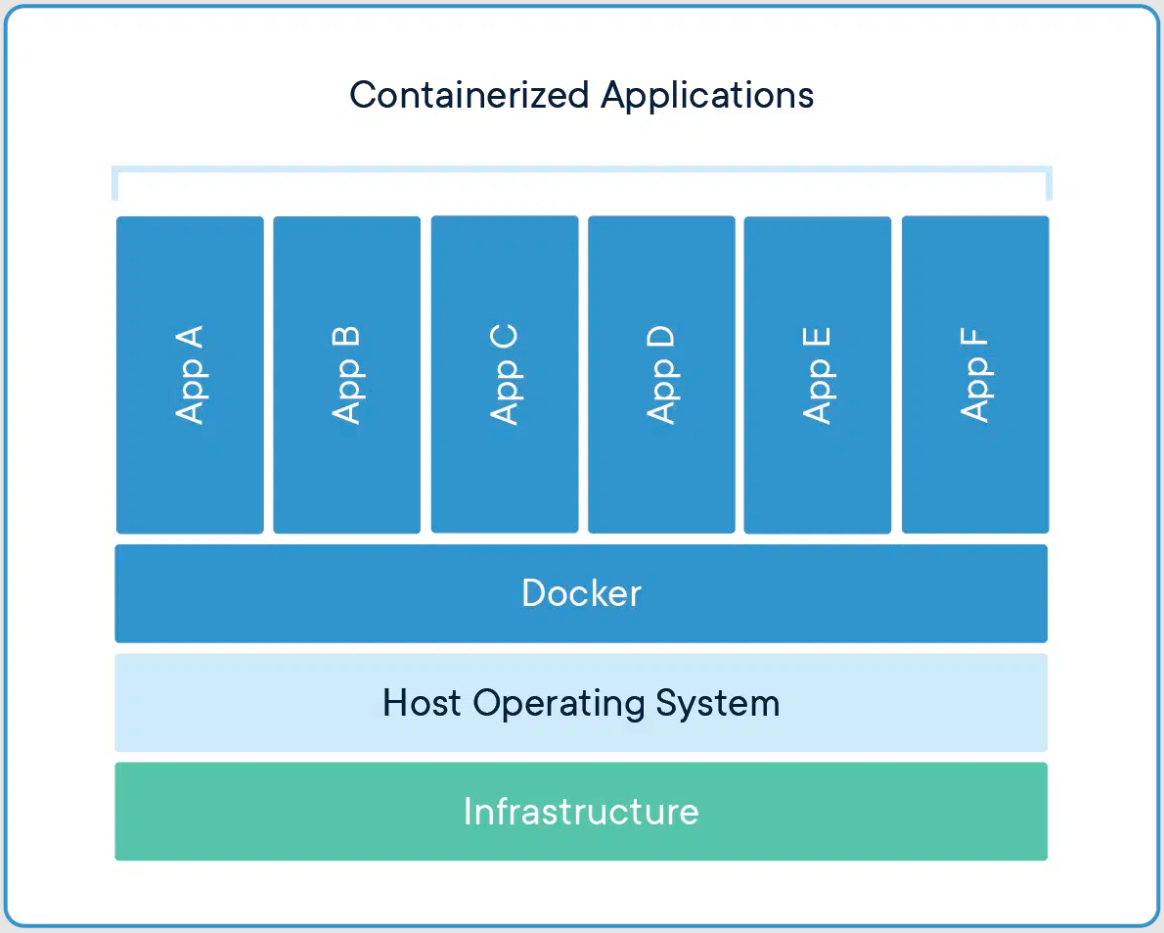
\includegraphics[width=0.8\textwidth]{pics/kontainerIlust.png}
	\caption{Ilustrasi kontainer \citep{docker_2022}}
	\label{fig:kontainer}
\end{figure}


\section{Docker}
\label{sec:dockerDef}
Docker merupakan salah satu cara untuk mengimplementasikan proses kontainerisasi. Docker diperkenalkan pada tahun 2013 dan dirilis untuk umum pada tahun 2014. Setelah kemunculannya penggunaan Docker menjadi sangat populer pada kalangan developer. Hal ini terjadi karena docker memiliki banyak keunggulan seperti: memiliki konfigurasi yang sederhana, tingkat keamanan yang baik, dan lain lain\citep{setiawan_2021}.
%-----------------------------------------------------------------------------%
\section{Kubernetes}
\label{sec:kubernetes}
%-----------------------------------------------------------------------------%
Kubernetes merupakan perangkat lunak sumber terbuka yang berguna untuk orkestrasi kontainer\citep{kubernetes}. Kubernetes dapat membantu banyak operasi seperti \textit{deployment, scaling deployment, mounting}, dan konfigurasi domain. Kontainer Docker dapat dikendalikan oleh Kubernetes.
%-----------------------------------------------------------------------------%
\section{Helm}
\label{sec:helmDef}
Helm merupakan manajer paket yang digunakan untuk mempermudah penggunaan Kubernetes\citep{merron_idowu_2020}. Dengan Helm, pengguna dapat mendefinisikan \textit{template} yang dapat dipakai untuk membuat proses modul \textit{deployment} Kubernetes menjadi lebih mudah. Definisi-definisi template beserta nilainya akan disimpan kedalam sebuah berkas yang dinamakan \code{helm chart}.
%-----------------------------------------------------------------------------%
\section{Terraform}
\label{sec:terraformDef}
Terraform adalah infrastructure as a code(IAAC) dimana pengguna dapat mendefinisikan spesifikasi \textit{deployment} pada kode\citep{terraform}. Kode tersebut kemudian akan dibaca oleh Terraform \textit{provider} yang akan melakukan \textit{deployment} sesuai dengan perintah kode. Terraform telah terintegrasi dengan banyak aplikasi seperti Kubernetes, Helm, Vault, dan fitur-fitur AWS.
%-----------------------------------------------------------------------------%
\section{Golang}
\label{sec:golang}
Go atau yang sering disebut Golang merupakan bahasa pemrograman yang dikembangkan oleh Google pada tahun 2009\citep{chris_2021}. Setelah dirilis, kepopuleran golang terus naik karena memiliki banyak keunggulan seperti: \textit{simple}, cepat, dan efisien. Golang digunakan untuk mengembangkan banyak aplikasi seperti Docker, Kubernetes, Helm, dan Vault.
%-----------------------------------------------------------------------------%
\section{Aplikasi Pihak ketiga}
\label{sec:aplikasiPihakKetiga}

Dalam dunia kerja, ada banyak aplikasi yang berjalan dan digunakan secara bersamaan. Aplikasi tersebut akan bekerja sama satu sama lain secara langsung maupun tidak langsung. Bagian ini akan membahas tentang aplikasi pihak ketiga yang akan diintegrasikan ke dalam aplikasi yaitu: Amazon S3, Amazon Kinesis, dan Vault.
%-----------------------------------------------------------------------------%
\subsection{Amazon S3}
\label{sec:amazonS3}

Amazon S3 merupakan solusi penyimpanan yang disediakan oleh Amazon\citep{chai_2021}. Amazon S3 digunakan untuk melakukan pencadangan dan penyimpanan data aplikasi pada Amazon Web Services. Amazon S3 didesain dengan sederhana untuk mempermudah proses integrasi dengan aplikasi.

%-----------------------------------------------------------------------------%
\subsection{Amazon Kinesis}
\label{sec:amazonKinesis}

Amazon Kinesis adalah message broker yang berfungsi untuk menerima data dalam bentuk \textit{stream}\citep{butts_2021}. Amazon Kinesis membantu pengguna memproses data yang masuk agar dapat diolah menjadi data yang dapat dianalisis. Setiap instance Amazon Kinesis dapat memilki banyak \textit{shards} yang masing-masingnya dapat menerima 1000 \textit{PUT request}.
%-----------------------------------------------------------------------------%
\subsection{Vault}
\label{sec:vault}

Vault merupakan sistem yang dirancang untuk dapat menyimpan rahasia secara aman dan memberikan akses kepada pihak yang berhak \citep{lugger_2020}. Rahasia yang dimaksud mencakup: \textit{password}, kunci API, kunci SSH, kunci RSA, dan lain lain. Rahasia yang tersimpan pada vault telah terenkripsi, sehingga meningkatkan keamanan dari penyimpanan tersebut.
%-----------------------------------------------------------------------------%
\section{\textit{Design Pattern}}
\label{sec:designPattern}
\textit{Design pattern} adalah solusi untuk banyak permasalahan dalam dunia pengembangan perangkat lunak\citep{shvets_2014dp}. \textit{Design pattern} bukanlah kode spesifik namun merupakan konsep umum dalam permasalahan yang spesifik. Bagian ini akan membahas beberapa \textit{design pattern} yang digunakan dalam aplikasi yang dikembangkan yaitu: \textit{Controller-Service-Repository}, dan \textit{Singleton}. 

%-----------------------------------------------------------------------------%
\subsection{\textit{Controller-Service-Repository}}
\label{sec:modelsViewController}

\textit{ControllerService-Repository} merupakan desain pattern yang didesain untuk memisahkan proses permintaan pada \textit{REST API}\citep{collings_2021}. Controller bertugas untuk membaca data dan mengubahnya menjadi data yang dapat dimengerti oleh \textit{service}. \textit{Service} berisi implementasi dari logika bisnis aplikasi. \textit{Repository} kode yang melakukan penyimpanan kedalam database.
%-----------------------------------------------------------------------------%
\subsection{\textit{Singleton}}
\label{sec:singleton}
\textit{Singleton} merupakan \textit{design pattern} yang didesain agar hanya ada satu \textit{instance} objek untuk setiap pemanggilan objek tersebut. Hal ini dilakukan agar tidak terjadinya \textit{memory leak} yang disebabkan oleh instansiasi objek yang terlalu banyak. Dengan menggunakan \textit{singleton}, pengguna hanya memiliki akses kepada \textit{getter} dari \textit{instance} tersebut yang akan mengembalikan objek jika objek tersebut sudah ada di memori, namun akan akan membuat objek baru jika objek tersebut belum ada\citep{shvets_2014st}.
%-----------------------------------------------------------------------------%
\section{Pekerjaan Terdahulu}
\label{sec:prevWork}

Terdapat pekerjaan serupa yang dikerjakan oleh \cite{microsoft_2019} yang mencoba untuk membuat API untuk melakukan \textit{deployment} Helm Chart melalui \textit{request HTTP}. Proyek ini dikembangkan mengunakan bahasa pemrograman Javascript. Sayangnya proyek ini sudah tidak lagi dikelola semenjak tahun 2019 dan kode sumbernya telah diarsipkan. 
\clearchapter
%-----------------------------------------------------------------------------%
\chapter{\babTiga}
\label{bab:3}
%-----------------------------------------------------------------------------%
Bab ini menjelaskan proses perancangan dari aplikasi yang dikembangkan penulis. Proses perancangan dimulai dari menjelaskan metode penelitian, analisis kebutuhan, identifikasi fitur, dan perancangan arsitektur aplikasi.


\section{Metode Penelitian}
\label{sec:metodePenelitian}

Gambar \ref{fig:alur-penelitian} menjelaskan alur umum dari penelitian yang akan dilakukan penulis. Berikut adalah penjelasan singkat mengenai setiap fase pada ilustrasi tersebut:

\begin{enumerate}
    \item \textbf{Studi Literatur}: Melakukan studi literatur awal mengenai helm dan penggunaan helm dan mengenai implementasi Helm API yang serupa. Penulis juga akan melakukan studi literatur mengenai integrasi Vault, Amazon Kinesis, dan Templating.
    \item \textbf{Analisis Kebutuhan}: Mengumpulkan kebutuhan dari pengguna. Kebutuhan didapatkan dari wawancara yang dilakukan oleh penulis kepada pengguna saat masa perancangan aplikasi.
    \item \textbf{Identifikasi Fitur}: Dari kebutuhan yang telah dikumpulkan selama masa analisis kebutuhan, akan dikumpulkan fitur yang akan dimiliki oleh aplikasi.
    \item \textbf{Perancangan Fungsi Aplikasi}: Akan dibuat daftar fungsi-fungsi yang dapat digunakan pada aplikasi.
    \item \textbf{Perancangan Arsitektur Lingkungan Kubernetes}: Penulis akan merancang skema arsitektur Kubernetes dimana aplikasi yang dikembangkan akan berjalan.
    \item \textbf{Perancangan Arsitektur Aplikasi}: Penulis akan merancang skema arsitektur aplikasi berdasarkan kebutuhan fitur yang telah dikumpulkan.
    \item \textbf{Implementasi Program}: Akan dilakukan implementasi aplikasi berdasarkan rancangan yang telah disusun pada tahapan analisis dan perancangan.
    \item \textbf{Implementasi Kebutuhan \textit{Deployment}}: Mengkonfigurasikan kebutuhan-kebutuhan yang diperlukan agar aplikasi yang telah dikembangkan dapat berjalan pada \textit{server}.
    \item \textbf{Proses \textit{Deployment}}: Penulis melakukan proses \textit{deployment} aplikasi kedalam lingkungan kerja milik PT Gudang Ada Globalindo.
    \item \textbf{Pengujian}: Penulis akan melakukan pengujian aplikasi dari kebutuhan yang telah dispesifikasikan.
\end{enumerate}

\begin{figure}
	\centering
	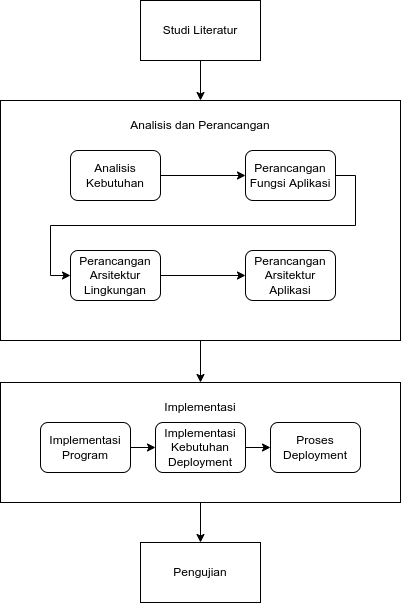
\includegraphics[width=0.8\textwidth]{pics/MetodePenelitian.png}
	\caption{Alur penelitian penulis}
	\label{fig:alur-penelitian}
\end{figure}

%-----------------------------------------------------------------------------%
\section{Analisis Kebutuhan}
\label{sec:analisisKebutuhan}
%-----------------------------------------------------------------------------%
Dikumpulkan kebutuhan melalui diskusi dengan \textit{user} yang dilakukan selama masa penelitian. Dari hasil diskusi tersebut, didapatkan kebutuhan pengguna dapat dilihat dari tabel berikut:

\begin{table}
    \centering
    \begin{tabular}{|c|p{12cm}|}
        \hline
        \multicolumn{1}{|c|}{Kode} & \multicolumn{1}{c|}{\textbf{Kebutuhan Pengguna (K)}} \\
        \hline
        K1 & Pengguna dapat melakukan \textit{deployment} satu atau lebih helm sekaligus. \\
        \hline
        K2 & Pengguna dapat melakukan \textit{deployment} pada \textit{namespace} Kubernetes yang berbeda-beda \\
        \hline
        K3 & Pengguna dapat membuat satu atau lebih Amazon Kinesis \textit{instance} sekaligus. \\
        \hline
        K4 & Pengguna akan melakukan banyak \textit{deployment} dengan spesifikasi yang mirip. \\
        \hline
        K5 & \textit{Repository} Helm Chart yang sedang dipakai harus tetap dipakai. \\
        \hline
        K6 & Pengguna dapat melakukan perubahan pada \textit{service} yang sudah di \textit{deploy}. \\
        \hline
        K7 & Pengguna dapat menghapus \textit{service} yang sudah di \textit{deploy}. \\
        \hline
        K8 & \textit{Service} yang dapat dihapus hanyalah \textit{service} yang di \textit{deploy} oleh aplikasi, bukan \textit{service} lain yang berada pada lingkungan yang sama \\
        \hline
        K9 & Pengguna dapat melihat detail dari \textit{service} yang sudah di \textit{deploy}. \\
        \hline
        K10 & Pengguna dapat melakukan \textit{deployment} aplikasi yang memiliki \textit{secret environment variable} tanpa mengetahui variabel tersebut. \\
        \hline
    \end{tabular}
    \caption{Identifikasi Kebutuhan}
    \label{tab:analisisKebutuhanPengguna}
\end{table}

\section{Identifikasi fitur}
\label{sec:identifikasiFitur}

Data dari tabel \ref{tab:analisisKebutuhanPengguna} dapat ditranformasikan menjadi spesifikasi yang diinginkan pada aplikasi yang akan dikembangkan. Hasil dari analisis tersebut akan dijadikan kebutuhan teknis yang dapat dilihat pada tabel \ref{tab:analisisFitur}:
\begin{table}
    \centering
    \begin{tabular}{|c|p{11cm}|p{1.5cm}|}
        \hline
         &  & \multicolumn{1}{|c|}{\textbf{Kode}} \\
        \multicolumn{1}{|c|}{\textbf{Kode}} &  \multicolumn{1}{c|}{\textbf{Kebutuhan Fitur Aplikasi (F)}} & \multicolumn{1}{|c|}{\textbf{Referensi}}\\
        & & \multicolumn{1}{|c|}{\textbf{K}} \\
        \hline
        F1 & Aplikasi memiliki fitur \textit{templating} yang dapat mengintegrasikan banyak \textit{deployment} sekaligus. & K1, K3, K4\\
        \hline
        F2 & Aplikasi dapat melayani proses \textit{deployment} Helm. & K1, K2\\
        \hline
        F3 & Aplikasi dapat melayani proses \textit{deployment} Amazon Kinesis. & K3\\
        \hline
        F4 & Aplikasi berintegrasi dengan Amazon S3 sebagai tempat penyimpanan Helm Chart. & K5\\
        \hline
        F5 & Terdapat \textit{persistence layer} yang dapat mencatat \textit{deployment}, perubahan \textit{deployment}, dan penghapusan \textit{deployment}. & K6, K7, K8, K9\\
        \hline        
    \end{tabular}
    \caption{Identifikasi Fitur}
    \label{tab:analisisFitur}
\end{table}
%-----------------------------------------------------------------------------%

\section{Perancangan Fungsi Aplikasi}
\label{sec:penggunaanAplikasi}

Aplikasi yang akan dikembangkan memiliki beberapa fitur yang telah dikumpulkan pada tabel \ref{tab:analisisFitur}. Fitur tersebut akan di akses oleh pengguna melalui beberapa fungsi. Bagian ini akan menjelaskan fungsi-fungsi yang dapat dipanggil oleh pengguna yang disediakan oleh aplikasi.

\subsection{Helm}
\label{sec:helmFeature}

Aplikasi yang dikembangkan harus dapat melakukan proses \textit{deployment} Helm. Adapun fungsi yang disediakan oleh aplikasi adalah sebagai berikut:

\begin{itemize}
    \item Membuat \textit{deployment} Helm.
    \item Melihat seluruh \textit{deployment} Helm.
    \item Melihat detail dari suatu \textit{deployment} Helm.
    \item Mengubah data dari suatu \textit{deployment} Helm.
    \item Menghapus suatu \textit{deployment} Helm.
\end{itemize}

\subsection{Kinesis}

Aplikasi yang dikembangkan harus dapat membuat \textit{instance} Amazon Kinesis. Adapun fungsi yang disediakan oleh aplikasi adalah sebagai berikut:

\begin{itemize}
    \item Membuat \textit{instance} Amazon Kinesis.
    \item Melihat seluruh \textit{instance} Amazon Kinesis.
    \item Melihat detail dari suatu \textit{instance} Amazon Kinesis.
    \item Mengubah data dari suatu \textit{instance} Amazon Kinesis.
    \item Menghapus suatu \textit{instance} Amazon Kinesis.
\end{itemize}

\subsection{Templating}

Aplikasi yang dikembangkan juga harus dapat membuat sistem \textit{templating} yang dapat melakukan \textit{deployment} Helm dan pembuatan \textit{instance} Amazon Kinesis. Aplikasi tersebut juga harus dapat mengakses variabel rahasia agar dapat mengamankan proses \textit{deployment}. Adapun fungsi yang disediakan oleh aplikasi adalah sebagai berikut:

\begin{itemize}
    \item Membuat definisi \textit{template deployment}.
    \item Melakukan \textit{deployment} berdasarkan \textit{template} yang telah didefinisikan.
    \item Melihat semua \textit{deployment}.
    \item Melihat detail dari sebuah \textit{deployment}.
    \item Mengubah \textit{deployment}.
    \item Menghapus \textit{deployment}.
\end{itemize}

\section{Perancangan Arsitektur Lingkungan Kubernetes}
\label{sec:perancanganEnvironment}
Aplikasi yang dikembangkan perlu di \textit{deploy} dan dikonfigurasikan sesuai kebutuhan pengguna. Aplikasi yang telah dikembangkan akan dikemas keladalam kontainer seperti gambar \ref{fig:aplikasiDiDalamKontainer}. 

\begin{figure}
	\centering
	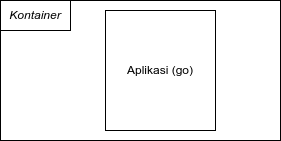
\includegraphics[width=0.5\textwidth]{pics/AplikasiDalamKontainer.png}
	\caption{Aplikasi di dalam kontainer}
	\label{fig:aplikasiDiDalamKontainer}
\end{figure}

Kontainer pada gambar \ref{fig:aplikasiDiDalamKontainer} akan diletakkan pada lingkungan Kubernetes yang akan dikendalikan seperti gambar \ref{fig:aplikasiDiDalamKubernetes}. 
\begin{figure}
	\centering
	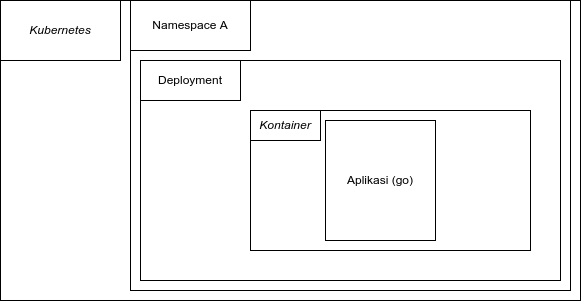
\includegraphics[width=0.6\textwidth]{pics/AplikasiDalamKubernetes.png}
	\caption{Kontainer berada di dalam \textit{environment} kubernetes}
	\label{fig:aplikasiDiDalamKubernetes}
\end{figure}

\subsection{Akses ke Aplikasi Pihak Ketiga}
Agar dapat berjalan dengan baik, aplikasi membutuhkan akses kepada \textit{database}, Vault Client, dan Amazon S3 Client milik GudangAda. Oleh karena itu perlu sambungan dari aplikasi ke masing masing klien. \textit{Credentials} untuk menghubungkan ke masing klien diberikan oleh \textit{serviceaccount} yang menempelkan \textit{credentials} tersebut ke \textit{environment} variabel pada kontainer aplikasi. Gambar \ref{fig:aplikasiMendapatCredentials} memperlihatkan kondisi aplikasi pada lingkungan Kubernetes setelah mendapat akses \textit{credentials} dan terhubung ke klien pihak ketiga.

\begin{figure}
	\centering
	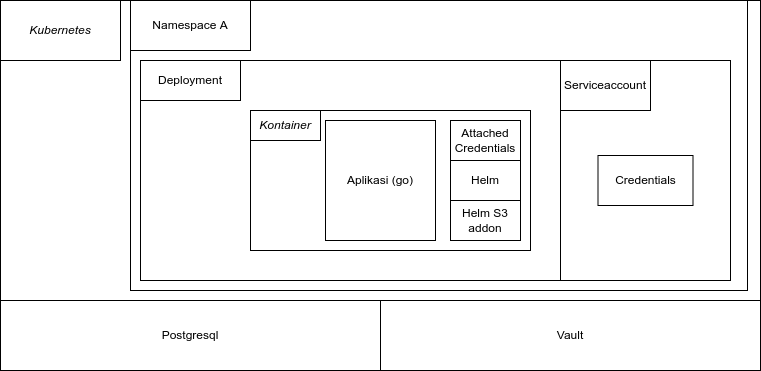
\includegraphics[width=0.75\textwidth]{pics/AplikasiMendapatCredentials.png}
	\caption{Aplikasi mendapat koneksi ke \textit{Database}, Vault \textit{client}, Amazon S3 \textit{Client}}
	\label{fig:aplikasiMendapatCredentials}
\end{figure}


\newpage

\subsection{Pengendalian \textit{Deployment} Pada Kubernetes}

Aplikasi perlu dapat mengendalikan banyak \textit{deployment} yang terdapat pada \textit{namespace} yang berbeda-beda. Oleh karena itu, \textit{serviceaccount} aplikasi perlu diberikan akses kepada \textit{namespace-namespace} yang akan dikendalikan.

\begin{figure}
	\centering
	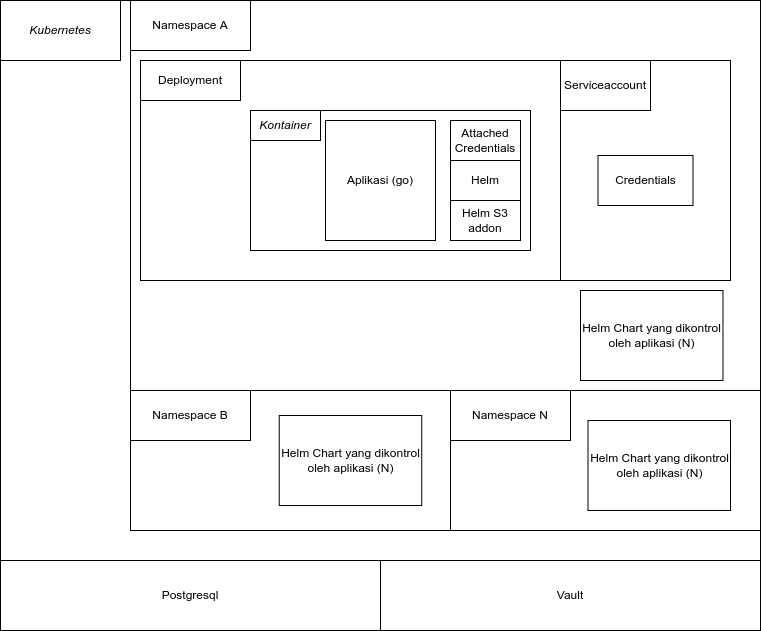
\includegraphics[width=0.85\textwidth]{pics/AplikasiMengontrolDeployment.png}
	\caption{Aplikasi mengontrol \textit{deployment}}
	\label{fig:aplikasiMengontrolDeployment}
\end{figure}

\newpage

\subsection{Akses Pengguna ke Aplikasi}

Agar dapat diakses oleh pengguna, perlu akses dari luar untuk dapat mengirimkan perintah ke aplikasi. Untuk memastikan orang yang dapat mengakses aplikasi merupakan orang yang berhak, dibutuhkan implementasi fitur otorisasi. Sayangnya, fitur otorisasi tidak termasuk ke dalam rancangan \textit{Minimum Viable Product}(MVP) aplikasi yang ditetapkan oleh perusahaan.

Sehingga pada penelitian kali ini, akses dari pengguna tidak dapat dilakukan dengan sambungan ke \textit{internet}. Akses ke aplikasi dilakukan dengan cara membuat \textit{port forward} dari \textit{Deployment} aplikasi ke perangkat pengguna setiap kali pengguna ingin mengakses aplikasi seperti gambar \ref{fig:arsitekturFinalAplikasi}. Pengguna yang ingin melakukan \textit{port forward} harus memiliki akses ke Kubernetes Cluster yang dikendalikan oleh aplikasi. Hal ini dilakukan untuk membatasi akses aplikasi ke pengguna yang berhak.


\begin{figure}
	\centering
	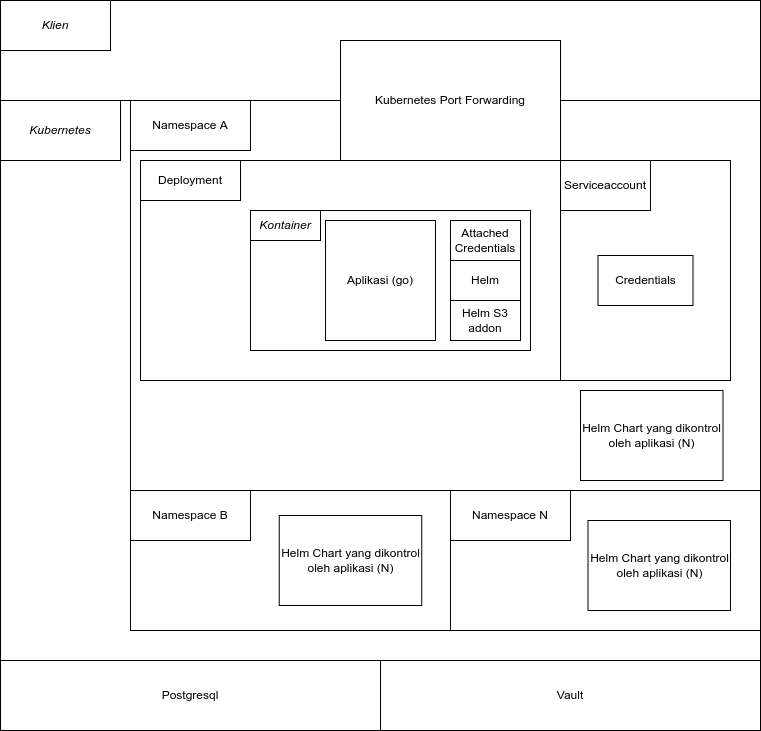
\includegraphics[width=1\textwidth]{pics/ArsitekturFinalAplikasi.png}
	\caption{Penggunaan aplikasi melalui \textit{port forwarding}}
	\label{fig:arsitekturFinalAplikasi}
\end{figure}



\section{Perancangan Arsitektur Aplikasi}
\label{sec:perancanganArsitektur}

Bagian ini menjelaskan mengenai desain aplikasi yang meliputi: justifikasi pemilihan teknologi, desain utama aplikasi, desain \textit{templating engine}, dan desain\textit{ secret engine}.

\subsection{Pemilihan Teknologi}
\label{sec:pemilihanTeknologi}
Penulis akan mengembangkan aplikasi menggunakan bahasa pemrograman Go. Pemilihan ini didasarkan karena hampir semua aplikasi pihak ketiga dikembangkan menggunakan Golang dan API disediakan dalam bentuk \textit{library} Go. Selain itu, sebagian besar \textit{Engineer} pada tim data GudangAda menggunakan bahasa pemrograman Go, sehingga mengembangkan aplikasi dengan menggunakan Go akan mempermudah pengembangan aplikasi ke depannya.

\subsection{Desain Utama Aplikasi}
\label{sec:desainUtamaAplikasi}
Aplikasi yang dikembangkan akan menggunakan arsitektur \textit{Controller-Service-Repository} dimana permintaan yang masuk akan diterima oleh \textit{router} yang kemudian akan diarahkan ke masing-masing \textit{controller} untuk diproses. Setelah masuk ke \textit{controller}, data dari permintaan akan di \textit{parse} untuk selanjutnya diarahkan ke \textit{services}. \textit{Services} akan menjalankan logika bisnis untuk mencatat dan verifikasi permintaan yang masuk. Setelah itu \textit{Sevices} akan memanggil \textit{repository} yang akan mengirimkan perintah \textit{deployment} kepada Helm API, \textit{database} dan/atau Amazon Kinesis API. Rancangan awal aplikasi dapat dilihat pada gambar \ref{fig:rancanganAwalAplikasi}.


\begin{figure}
	\centering
	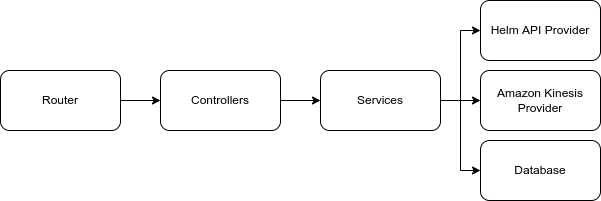
\includegraphics[width=1\textwidth]{pics/rancanganAplikasiAwal.png}
	\caption{Desain Aplikasi}
	\label{fig:rancanganAwalAplikasi}
\end{figure}

Di dalam \textit{service} terdapat \textit{templating engine} yang dapat melakukan \textit{parsing request} asli ke dalam spesifikasi akhir dan \textit{Vault engine} yang akan memasukkan variabel rahasia ke dalam aplikasi.

\subsection{\textit{Templating Engine}}
\label{sec:templatingEngine}
Untuk memenuhi kebutuhan K4, dibutuhkan sistem \textit{template} dimana pengguna dapat mendefinisikan sebuah \textit{template} pada aplikasi dan melakukan \textit{deployment} berdasarkan \textit{template} tersebut.\textit{ Templating engine} milik Golang akan digunakan untuk melakukan \textit{templating} pada aplikasi yang dikerjakan. 

\begin{figure}
	\centering
	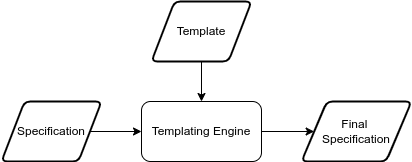
\includegraphics[width=0.7\textwidth]{pics/TemplatingEngine.png}
	\caption{Alur kerja \textit{templating engine}}
	\label{fig:alurTemplatingEngine}
\end{figure}

Pada gambar \ref{fig:alurSecretEngine} dapat dilihat bahwa dibutuhkan \textit{template} dan spesifikasi \textit{deployment} untuk mendapatkan spesifikasi akhir. Pengguna dapat membuat definisi \textit{template} yang akan ditambahkan kedalam \textit{database}. Setelah itu, pengguna dapat mengirimkan spesifikasi dari \textit{deployment} berdasarkan \textit{template} yang telah didefinisikan. Sebagai contoh, jika ada definisi \textit{template} \ref{code:templateFile} dan spesifikasi \textit{deployment} \ref{code:templateValue}, maka akan terbentuk \ref{code:finalTemplate} yang akan dikirimkan kepada Helm API untuk dibuatkan \textit{deployment}.

\begin{lstlisting}[frame=single,caption={Contoh file \textit{template}},label={code:templateFile}]
chart:
- release_name: {{ .Values.name }}
  name: {{ .Values.chart.name }}
  namespace: {{ .Values.namespace }}
  version: {{ .Values.chart.version }}
\end{lstlisting}

\begin{lstlisting}[frame=single,caption={Contoh nilai yang dipakai},label={code:templateValue}]
name: regular-deployment
namespace: default
chart:
    name: nginx
    version: 1.0.0
\end{lstlisting}

\begin{lstlisting}[frame=single,caption={Hasil akhir \textit{template}},label={code:finalTemplate}]
chart:
- release_name: regular-deployment
  name: nginx
  namespace: default
  version: 1.0.0
\end{lstlisting}

\subsection{Secret Engine}
\label{sec:vaultEngine}

Spesifikasi \textit{deployment} sering kali mengandung variabel rahasia yang sebaiknya tidak diketahui oleh banyak orang. Oleh karena itu, variabel tersebut disembunyikan pada Vault yang aman dan memiliki akses yang terbatas. Aplikasi membutuhkan cara agar dapat mendapatkan variabel tersebut tanpa diketahui nilainya oleh orang yang melakukan proses \textit{deployment}.

Untuk memenuhi kebutuhan di atas, dibutuhkan integrasi dengan Vault dimana aplikasi dapat mengakses variabel rahasia yang tersimpan tanpa campur tangan langsung dari pengguna. Pengguna hanya perlu memberikan alamat dari variabel rahasia dan aplikasi akan mengakses variabel tersebut. 

\begin{figure}
	\centering
	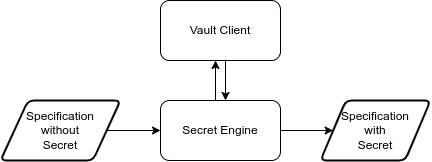
\includegraphics[width=0.7\textwidth]{pics/SecretEngine.png}
	\caption{Alur kerja \textit{secret engine}}
	\label{fig:alurSecretEngine}
\end{figure}

Alur kerja\textit{ secret engine} dapat dilihat pada gambar \ref{fig:alurSecretEngine}. Sebagai contoh, pengguna akan membuat \textit{template} terlebih dahulu seperti kode \ref{code:secretTemplate} dan pengguna akan memberikan alamat variabel pada Vault pada kode \ref{code:secretValue}, jika pada Vault terdapat \textit{key} 'kv/data/devops/regular-deployment' dan \textit{secret} 'DB-password' yang bernilai 'super-secret-password', maka aplikasi akan menggantikan nilai '.Values.secret.Vault.DBPass' menjadi 'super-secret-password' seperti kode \ref{code:secretFinal}.

\begin{lstlisting}[frame=single,caption={Contoh penggunaan \textit{secret} pada template},label={code:secretTemplate}]
name: regular-deployment
namespace: default
chart:
    name: nginx
    version: 1.0.0
    values:
        databasePassword: {{ .Values.secret.Vault.DBPass }}
\end{lstlisting}

\begin{lstlisting}[frame=single,caption={Contoh penggunaan \textit{secret} pada nilai yang dipakai},label={code:secretValue}]
secret:
  Vault:
    DBPass: kv/data/devops/regular-deployment:DB-password
\end{lstlisting}

\begin{lstlisting}[frame=single,caption={Contoh penggunaan \textit{secret} pada nilai yang dipakai},label={code:secretFinal}]
secret:
  Vault:
    DBPass: super-secret-password
\end{lstlisting}



\clearchapter
%-----------------------------------------------------------------------------%
\chapter{\babEmpat}
\label{bab:4}
%-----------------------------------------------------------------------------%
Bab ini menjelaskan secara rinci tahapan yang penulis lakukan dalam melakukan
proses implementasi berdasarkan rancangan serta analisis yang telah dilakukan
pada bab sebelumnya. Proses yang penulis lakukan pada tahapan implementasi
antara lain: implementasi program, implementasi kebutuhan \textit{deployment}, dan
proses \textit{deployment}.

\section{Implementasi Aplikasi}
\label{sec:implementasiAplikasi}
Aplikasi yang telah dirancang pada \ref{sec:perancanganArsitektur} akan diimplementasikan. Bagian ini akan menjelaskan contoh dari kode yang merepresentasikan alur kerja aplikasi. Berkas sumber kode yang lengkap dapat dilihat pada lampiran \ref{appendix:hasilAplikasi}.

Implementasi program dimulai dengan melakukan inisiasi proyek pada Golang dengan melakukan \code{go mod init project-source}, dimana \code{project-source} merupakan lokasi sumber kode pada repositori GitHub milik GudangAda. Untuk memastikan repositori lebih teratur, penulis akan mengikuti konvensi dari \cite{golang-standards_2022} sebagai paduan untuk meletakkan berkas kode.

\subsection{Implementasi Bagian Utama Program}
\label{sec:maingo}
Kode utama pada aplikasi berisi inisiasi untuk membaca berkas konfigurasi, inisiasi \textit{router}, dan inisiasi \textit{HTTP listener}. Pada kode utama inilah \textit{server} berjalan untuk mendengarkan permintaan \textit{HTTP} dari \textit{host} dan \textit{port} yang telah diberikan.

\begin{lstlisting}[frame=single,language=Go,caption={Kode utama pada aplikasi yang dikembangkan},label={code:maingo}]
func main() {
	var rt routes.Route

	appConfigs, err := configs.InitAppConfigs()
	if err != nil {
		panic(err)
	}

	router := rt.Init(*appConfigs)

	var gracefulStop = make(chan os.Signal)
	signal.Notify(gracefulStop, syscall.SIGTERM)
	signal.Notify(gracefulStop, syscall.SIGINT)
	go func() {
		sig := <-gracefulStop
		fmt.Printf("caught sig: %+v", sig)
		fmt.Println("Wait for 2 second to finish processing")
		time.Sleep(2 * time.Second)
		os.Exit(0)
	}()

	headersOK := handlers.AllowedHeaders([]string{"X-Requested-With", "Content-Type", "NAME", "MODULE_NAME", "VERSION", "ON_FAILURE"})
	originsOK := handlers.AllowedOrigins([]string{"*"})
	methodsOK := handlers.AllowedMethods([]string{"GET", "POST", "OPTIONS", "DELETE", "PUT"})
	host := appConfigs.Server.Host
	port := strconv.Itoa(appConfigs.Server.Port)
	fmt.Println("Server served at port " + port)
	if err := http.ListenAndServe(host+":"+port, handlers.CORS(originsOK, headersOK, methodsOK)(router)); err != nil {
		log.Fatal("Unable to start service: " + err.Error())
	}
}
\end{lstlisting}

\subsection{Membaca Berkas Konfigurasi}
\label{sec:readConfig}
Nilai-nilai penting seperti \textit{credentials} ke \textit{Database}, pengaturan \textit{server}, \textit{password} ke Vault perlu didapatkan saat aplikasi pertama kali berjalan. Oleh karena itu, dibutuhkan sebuah fungsi yang dapat membaca \textit{file} konfigurasi saat aplikasi pertama kali dijalankan. Fungsi tersebut ada pada kode \ref{code:configInit}.

fungsi \code{InitAppConfig} pada kode \ref{code:configInit} bertugas untuk membaca konfigurasi dari \textit{environment} \textit{variable} atau dari \textit{file} konfigurasi. Data yang dibaca akan dimasukkan ke dalam sebuah variabel yang didefinisikan pada kode \ref{code:configStruct}. Variabel yang didapatkan akan dikembalikan ke fungsi utama pada kode \ref{code:maingo} untuk disebarkan lagi ke masing masing fungsi yang membutuhkannya.

\begin{lstlisting}[frame=single,language=Go,caption={\textit{Struct} yang berisi definisi variabel konfigurasi aplikasi},label={code:configStruct}]
type AppConfigs struct {
	Server     ServerConfig `yaml:"server"`
	Database   DBConfig     `yaml:"database"`
	Kubernetes AuthConfig   `yaml:"Kubernetes"`
	Vault      VaultConfig  `yaml:"vault"`
	ChartRepo  ChartRepo    `yaml:"chartRepo"`
}
\end{lstlisting}

\begin{lstlisting}[frame=single,language=Go,caption={Fungsi untuk membaca berkas konfigurasi},label={code:configInit}]
func InitAppConfigs() (*AppConfigs, error) {
	var appConfigs AppConfigs

	err := cleanenv.ReadEnv(&appConfigs)
	if err != nil {
		return nil, err
	}

	configFile := "config.yaml"
	if _, err := os.Stat(configFile); os.IsNotExist(err) {
		return &appConfigs, nil
	}

	err = cleanenv.ReadConfig(configFile, &appConfigs)
	if err != nil {
		return nil, err
	}

	return &appConfigs, nil
}
\end{lstlisting}

\subsection{Implementasi Koneksi ke Aplikasi Pihak Ketiga Pada Aplikasi}

Sesuai rancangan \ref{sec:aplikasiPihakKetiga}, aplikasi akan terkoneksi ke aplikasi pihak ketiga. Koneksi ke aplikasi pihak ketiga harus diinisiasikan terlebih dahulu sebelum dapat dipakai. Koneksi yang harus dibuat adalah koneksi ke \textit{Database}, Helm, Vault, dan Amazon Kinesis. Masing-masing inisiasi dilakukan dengan cara yang berbeda beda. Bagian ini akan menjelaskan cara aplikasi membuat koneksi ke masing masing aplikasi pihak ketiga.

\subsubsection{Inisiasi Koneksi ke \textit{Database}}
\label{sec:initDB}

Fungsi untuk mendapatkan koneksi ke \textit{database} yang didefinisikan pada kode \ref{code:databaseInit} diimplementasikan dengan \textit{design pattern singleton}. Inisiasi \textit{database} dilakukan dengan membuat koneksi ke \textit{database}, dan melakukan migrasi terhadap semua \textit{models} yang diperlukan.
\begin{lstlisting}[frame=single,language=Go,caption={Fungsi untuk inisiasi koneksi ke \textit{Database}},label={code:databaseInit}]
var database *gorm.DB

func GetDB(config configs.DBConfig) (*gorm.DB, error) {
	if database != nil {
		return database, nil
	}
	var err error
	dsn := fmt.Sprintf(
		"host=%s user=%s password=%s dbname=%s port=%d sslmode=allow TimeZone=UTC",
		config.Host,
		config.User,
		config.Password,
		config.Name,
		config.Port,
	)
	database, err = gorm.Open(postgres.Open(dsn), &gorm.Config{
		Logger: newLogger(),
	})
	if err != nil {
		return nil, err
	}

	err = database.AutoMigrate(&models.ChartRelease{})
	if err != nil {
		return nil, err
	}

	err = database.AutoMigrate(&models.Module{})
	if err != nil {
		return nil, err
	}

	err = database.AutoMigrate(&models.ModuleRelease{})
	if err != nil {
		return nil, err
	}

	err = database.AutoMigrate(&models.Kinesis{})
	if err != nil {
		return nil, err
	}

	return database, nil
}
\end{lstlisting}

\subsubsection{Inisiasi Koneksi ke Helm}
\label{sec:initHelm}

Khusus untuk koneksi ke Helm, tidak dapat diimplementasikan dengan \textit{singleton}. Hal ini terjadi karena pada kebutuhan K2, aplikasi harus dapat melakukan \textit{deployment} pada \textit{namespace} yang berbeda-beda. Namun, sebuah objek helm \textit{client} hanya dapat melakukan \textit{deployment} pada sebuah \textit{namespace} yang telah ditentukan sebelumnya. Oleh karena itu, akan dibuat N buah objek Helm \textit{Client} dimana N adalah jumlah \textit{namespace} yang dapat dikendalikan yang telah ditentukan pada inisiasi program melalui berkas konfigurasi.

Ada dua cara untuk mendapatkan akses ke helm. Cara pertama adalah melalui \textit{file} kubeconfig, cara ini biasanya dilakukan pada masa pengembangan di \textit{environment} lokal. Cara kedua adalah melalui \textit{serviceaccount} yang dihubungkan oleh Kubernetes, cara ini biasanya dilakukan untuk \textit{environment} \textit{production}.

\begin{lstlisting}[frame=single,language=Go,caption={Fungsi untuk inisiasi koneksi ke Helm},label={code:helmInit}]
func GenerateHelmClient(authConfig configs.AuthConfig) (map[string]helm.Client, error) {
	helmClient := map[string]helm.Client{}
	var config *rest.Config
	var err error

	switch authConfig.Method {
	case "kubeconfig":
		var kubeconfig *string
		if home := homedir.HomeDir(); home != "" {
			kubeconfig = flag.String("kubeconfig", filepath.Join(home, ".kube", "config"), "(optional) absolute path to the kubeconfig file")
		} else {
			kubeconfig = flag.String("kubeconfig", "", "absolute path to the kubeconfig file")
		}
		flag.Parse()

		config, err = clientcmd.BuildConfigFromFlags("", *kubeconfig)
		if err != nil {
			return nil, err
		}
	case "service-account":
		config, err = rest.InClusterConfig()
		if err != nil {
			panic(err.Error())
		}
	}

	for _, namespace := range authConfig.AvailableNamespace {
		opt := &helm.RestConfClientOptions{
			Options: &helm.Options{
				Namespace: namespace,
			},
			RestConfig: config,
		}

		helmClientTmp, err := helm.NewClientFromRestConf(opt)
		if err != nil {
			panic(err)
		}

		helmClient[namespace] = helmClientTmp
	}
	return helmClient, nil
}
\end{lstlisting}

\subsubsection{Inisiasi Koneksi ke Vault}
\label{sec:initVault}

Fungsi untuk mendapatkan koneksi ke Vault yang didefinisikan pada kode \ref{code:vaultInit} diimplementasikan dengan \textit{design pattern singleton}. Inisiasi \textit{database} dilakukan dengan membuat koneksi ke \textit{login} ke \textit{server} milik Vault. Ada dua cara untuk mendapatkan akses, yaitu melalui Kubernetes Service Account dan memasukkan \textit{password}. Penggunaan \textit{login} melalui Kubernetes Service Account biasanya dilakukan pada \textit{environment production}, sedangkan penggunaan \textit{login} melalui \textit{password} dilakukan untuk pengembangan aplikasi dalam \textit{environment local}.

\begin{lstlisting}[frame=single,language=Go,caption={Fungsi untuk inisiasi koneksi ke Vault},label={code:vaultInit}]
var vaultClient *api.Client

func GetVaultSecret(vaultConfig configs.VaultConfig) (*api.Client, error) {
	if vaultClient != nil {
		return vaultClient, nil
	}
	config := api.DefaultConfig()

	config.Address = vaultConfig.URL

	vaultClient, err := api.NewClient(config)
	if err != nil {
		return nil, err
	}

	var auth api.AuthMethod

	switch vaultConfig.AuthMethod {
	case "service-account":
		auth, err = Kubernetes.NewKubernetesAuth(
			vaultConfig.KubeMethod.RoleName,
			Kubernetes.WithMountPath(vaultConfig.KubeMethod.MountPath),
		)
		if err != nil {
			return nil, fmt.Errorf("unable to initialize Kubernetes auth method: %w", err)
		}
	case "userpass":
		auth, err = userpass.NewUserpassAuth(
			vaultConfig.UserPassMethod.Username,
			&userpass.Password{FromString: vaultConfig.UserPassMethod.Password},
		)
		if err != nil {
			return nil, fmt.Errorf("unable to initialize UserPass auth method: %w", err)
		}
	}

	authInfo, err := vaultClient.Auth().Login(context.TODO(), auth)
	if err != nil {
		return nil, fmt.Errorf("unable to log in with auth: %w", err)
	}
	if authInfo == nil {
		return nil, fmt.Errorf("no auth info was returned after login")
	}

	return vaultClient, nil
}
\end{lstlisting}

\subsubsection{Inisiasi Koneksi ke Amazon Kinesis}
\label{sec:initKinesis}

Fungsi untuk mendapatkan koneksi ke Amazon Kinesis yang didefinisikan pada kode \ref{code:kinesisInit} diimplementasikan dengan \textit{design pattern singleton}. Inisiasi objek dilakukan dengan membaca \textit{environment variable} atau dari \textit{serviceaccount}. Proses tersebut dilakukan secara otomatis oleh API yang disediakan oleh Amazon.

\begin{lstlisting}[frame=single,language=Go,caption={Fungsi untuk inisiasi Koneksi ke Amazon Kinesis},label={code:kinesisInit}]
var kinesisClient *kinesis.Client

func GetKinesisClient() (*kinesis.Client, error) {
	if kinesisClient != nil {
		return kinesisClient, nil
	}
	cfg, err := config.LoadDefaultConfig(context.TODO())
	if err != nil {
		return nil, err
	}
	kinesisClient = kinesis.NewFromConfig(cfg)
	return kinesisClient, nil
}
\end{lstlisting}

\subsection{Implementasi \textit{Routing} Aplikasi}
\label{sec:router}

Fungsi \textit{routing} pada aplikasi dimulai dengan melakukan inisiasi semua objek yang dibutuhkan yaitu Helm(fungsi pada kode \ref{code:helmInit}), Kinesis(fungsi pada kode \ref{code:kinesisInit}), \textit{Database}(fungsi pada kode \ref{code:databaseInit}), dan Vault(fungsi pada kode \ref{code:vaultInit}) pada kode \ref{code:clientInit}.
\begin{lstlisting}[frame=single,language=Go,caption={Pemanggilan fungsi inisiasi ke \textit{Database}, Helm, Vault, dan Amazon Kinesis},label={code:clientInit}]
helmClient, err := helm.GenerateHelmClient(config.Kubernetes)
if err != nil {
	panic(err)
}

chartRepo := helm.GetChartRepo(config.ChartRepo)

kinesisClient, err := kinesis.GetKinesisClient()
if err != nil {
	panic(err)
}

database, err := database.GetDB(config.Database)
if err != nil {
	panic(err)
}

vault, err := vault.GetVaultSecret(config.Vault)
if err != nil {
	panic(err)
}
\end{lstlisting}
Objek yang berfungsi sebagai koneksi ke aplikasi pihak ketiga tersebut akan dipakai sebagai dependensi dari objek \textit{repository}, \textit{service}, dan \textit{controller} yang berada pada kode  \ref{code:controllerServicesRepositoryInit}. 

\begin{lstlisting}[frame=single,language=Go,caption={Inisiasi \textit{Controller}, \textit{Service}, dan \textit{Repository}},label={code:controllerServicesRepositoryInit}]
defaultNamespace := config.Kubernetes.DefaultNamespace

moduleRepository := repositories.InitModuleRepository(database)

chartProvider := repositories.InitChartProvider(helmClient, database, defaultNamespace, chartRepo)
kinesisProvider := repositories.InitKinesisProvider(database, kinesisClient)

vaultSecretProvider := repositories.InitVaultSecretProvider(vault)

componentProviders := map[string]repositories.Providers{
	"chart":   chartProvider,
	"kinesis": kinesisProvider,
}

secretProviders := map[string]repositories.SecretProviders{
	"vault": vaultSecretProvider,
}

chartService := services.InitChartService(chartProvider)
kinesisService := services.InitKinesisService(kinesisProvider)
moduleService := services.InitModuleService(moduleRepository, componentProviders, secretProviders)

chartController := controllers.InitChartController(chartService)
kinesisController := controllers.InitKinesisController(kinesisService)
moduleController := controllers.InitModuleController(moduleService)
\end{lstlisting}

Terakhir, \textit{router} akan diinisiasikan dan dipakai untuk memisahkan permintaan \textit{HTTP} yang masuk berdasarkan \textit{method} dan \textit{path} dari \textit{URL} nya. \textit{Router} yang telah diinisiasi dan didefinisikan pembagian alamatnya akan dikembalikan ke kode \ref{code:maingo} untuk \textit{dibuatkan HTTP listener}.

\begin{lstlisting}[frame=single,language=Go,caption={Inisiasi dan penggunaan \textit{Router}},label={code:routerInit}]
router := mux.NewRouter().StrictSlash(false)

router.HandleFunc("/chart", chartController.Release).Methods(http.MethodPost)
router.HandleFunc("/chart", chartController.GetAllReleaseName).Methods(http.MethodGet)
router.HandleFunc("/chart/{chart-name}", chartController.GetReleaseDetail).Methods(http.MethodGet)
router.HandleFunc("/chart/{chart-name}", chartController.UpdateRelease).Methods(http.MethodPut)
router.HandleFunc("/chart/{chart-name}", chartController.RemoveRelease).Methods(http.MethodDelete)

router.HandleFunc("/kinesis", kinesisController.Release).Methods(http.MethodPost)
router.HandleFunc("/kinesis", kinesisController.GetAllReleaseName).Methods(http.MethodGet)
router.HandleFunc("/kinesis/{kinesis-name}", kinesisController.GetReleaseDetail).Methods(http.MethodGet)
router.HandleFunc("/kinesis/{kinesis-name}", kinesisController.UpdateRelease).Methods(http.MethodPut)
router.HandleFunc("/kinesis/{kinesis-name}", kinesisController.RemoveRelease).Methods(http.MethodDelete)

router.HandleFunc("/module", moduleController.AddModule).Methods(http.MethodPost)
router.HandleFunc("/module/release", moduleController.AddModuleRelease).Methods(http.MethodPost)
router.HandleFunc("/module/release", moduleController.GetAllReleaseName).Methods(http.MethodGet)
router.HandleFunc("/module/release/{release-name}", moduleController.GetReleaseDetail).Methods(http.MethodGet)
router.HandleFunc("/module/release/{release-name}", moduleController.UpdateModuleRelease).Methods(http.MethodPut)
router.HandleFunc("/module/release/{release-name}", moduleController.DeleteModuleRelease).Methods(http.MethodDelete)

return router
\end{lstlisting}

\subsection{Implementasi \textit{Controller} Aplikasi}
\label{sec:controller}

\textit{Controller} berfungsi untuk membaca permintaan dari pengguna dan mengubah datanya menjadi data yang dapat dimengerti oleh aplikasi. Sebagai contoh, pada kode \ref{code:controller}, \textit{controller} akan melakukan \textit{parsing request body} dan \textit{header} dan memasukkan datanya ke dalam objek \code{module}, \code{module\_release}, dan \code{delete\_on\_fail}. Kemudian, ketiga objek tersebut akan dijadikan sebagai parameter dari fungsi pada \textit{layer service}s. Data yang kembali dari \textit{service} akan dikembalikan kepada pengguna dalam bentuk \textit{HTTP response}.

\begin{lstlisting}[frame=single,language=Go,caption={Contoh Fungsi \textit{Controller}},label={code:controller}]
func (h *ModuleController) AddModuleRelease(res http.ResponseWriter, req *http.Request) {
	requestBody := requests.ModuleRelease{}
	val, err := ioutil.ReadAll(req.Body)
	requestBody.Name = req.Header.Get("NAME")
	requestBody.ModuleName = req.Header.Get("MODULE_NAME")
	requestBody.Version = req.Header.Get("VERSION")
	requestBody.Values = string(val)
	requestBody.DeleteOnFail = req.Header.Get("ON_FAILURE")
	if err != nil {
		helpers.Response(res, 400, nil, "error", err.Error())
		return
	}
	if requestBody.IsEmpty() {
		helpers.Response(res, 400, nil, "error", "cannot process empty request")
		return
	}

	module, moduleRelease, deleteOnFail := requestBody.TransformToModels(true)

	err = h.moduleService.ReleaseModule(module, moduleRelease, deleteOnFail)
	if err != nil {
		helpers.Response(res, 400, nil, "error", err.Error())
		return
	}

	helpers.Response(res, 200, nil, "success", "-")
}
\end{lstlisting}

\subsection{Implementasi Service Aplikasi}
\label{sec:serviceImpl}

\textit{Service} berisi logika bisnis yang diperlukan oleh aplikasi untuk validasi, dan pencatatan data. Sebagai contoh, kode \ref{code:service} berisi fungsi untuk melakukan \textit{deployment} pada \textit{template}. Fungsi tersebut memiliki alur kerja seperti berikut.
\begin{enumerate}
    \item Pada baris 2-5 akan dilakukan pengecekan apakah \textit{template} yang dimaksud ada.
    \item Pada baris 7-9 akan dilakukan inisiasi data-data \textit{deployment}.
    \item Pada baris 11-20 akan dilakukan \textit{templating} untuk mendapatkan spesifikasi final dari aplikasi.
    \item Pada baris 22-25 akan dilakukan pencatatan ke \textit{database} tentang \textit{deployment} yang sedang dilakukan.
    \item Pada baris 27-32 akan dilakukan pengecekan apakah \textit{interface} pengendali \textit{deployment} yang akan dilakukan \textit{deployment}(Helm, atau Amazon Kinesis) sudah diimplementasikan. Hal ini dilakukan untuk menghindari \code{nilPointerException} pada kasus \textit{interface deployment} yang belum diimplementasikan.
    \item Pada baris 34-50 dilakukan pemrosesan data untuk memastikan data tersebut siap untuk di \textit{deploy}. Detail untuk masing masing operasi kadang berbeda-beda. Oleh karena itu, tahapan ini dilakukan pada \textit{layer repository} masing masing pengendali \textit{deployment}.
    \item Pada baris 52-67 dilakukan proses \textit{deployment} untuk masing masing komponen yang harus di \textit{deploy}.
\end{enumerate}
Potongan kode \ref{code:service}  merupakan contoh fungsi membuat \textit{deployment} pada \textit{layer service}. Jika ingin melihat keseluruhan kode, dapat dilihat pada lampiran \ref{appendix:hasilAplikasi} bagian \code{internal/services/module\_service.go}.

\begin{lstlisting}[frame=single,language=Go,caption={Contoh Fungsi \textit{Service}},label={code:service}]
func (m ModuleService) ReleaseModule(module models.Module, release models.ModuleRelease, deleteOnFail bool) error {
	module, err := m.moduleRepository.GetModule(module.Name, module.Version)
	if err != nil {
		return err
	}

	release.ModuleID = module.ID
	release.ModuleName = module.Name
	release.Revision = 1

	finalSpec, err := m.applyChartTemplate(module, module.Spec, release)
	if err != nil {
		return err
	}

	var spec map[string][]interface{}
	err = yaml.Unmarshal([]byte(finalSpec), &spec)
	if err != nil {
		return err
	}

	release, err = m.moduleRepository.InsertModuleRelease(release)
	if err != nil {
		return err
	}

	for handler := range spec {
		if _, ok := m.providers[handler]; !ok {
			err := errors.New("component handler not implemented")
			return err
		}
	}

	for handler, components := range spec {
		for i, component := range components {
			spec[handler][i], err = m.providers[handler].Convert(component)
			if err != nil {
				return err
			}
		}
	}

	for handler, components := range spec {
		for i := range components {
			spec[handler][i], err = m.providers[handler].PreProcess(spec[handler][i], nil, module, release)
			if err != nil {
				return err
			}
		}
	}

	for handler, components := range spec {
		for _, component := range components {
			err = m.providers[handler].InstallComponent(component)
			if err != nil {
				if deleteOnFail {
					m.providers[handler].UninstallComponent(component)
					m.forceDelete(release)
				}
				return err
			}
			err = m.providers[handler].Add(component)
			if err != nil {
				return err
			}
		}
	}

	return nil
}
\end{lstlisting}

\subsection{Implementasi \textit{Templating} dan Vault}
\label{sec:template}

Fitur \ref{sec:templatingEngine} dan \ref{sec:vaultEngine} akan diimplementasikan pada bagian ini. Pada kode \ref{code:service} akan dipanggil fungsi \code{applyChartTemplate} yang akan diimplementasikan oleh kode \ref{code:template}. Fungsi tersebut akan mengumpulkan semua variabel yang akan dipakai sebagai data untuk \textit{template} menjadi satu variabel untuk mempermudah pekerjaan golang \textit{templating engine}. Setelah itu, variabel rahasia yang berada pada bagian \code{secret}\footnote{lihat kode \ref{code:secretValue}} pada data akan digantikan dengan nilai rahasia yang tersimpan pada \textit{vault}. Lalu, \textit{templating engine} akan mengganti data \textit{template} menjadi data akhir berdasarkan nilai \textit{template} yang telah dibuat.

\begin{lstlisting}[frame=single,language=Go,caption={Fungsi \textit{Template} dan Vault},label={code:template}]
func (h *ModuleService) applyChartTemplate(chart models.Module, chartTemplate string, release models.ModuleRelease) (string, error) {
	templateVal := models.ModuleTemplate{
		Module:  chart.Name,
		Version: chart.Version,
		Release: release.Name,
	}
	err := yaml.Unmarshal([]byte(release.Values), &templateVal.Values)
	if err != nil {
		return "", err
	}

	if secret, ok := templateVal.Values["secret"]; ok {
		parsedSecret := make(map[string]map[string]interface{})
		mappedSecret := secret.(map[string]interface{})
		for secretProviderName, rawSecret := range mappedSecret {
			if _, ok := h.secretProviders[secretProviderName]; !ok {
				err := errors.New("component handler not implemented")
				return "", err
			}

			secretProvider := h.secretProviders[secretProviderName]
			parsedRawSecret := rawSecret.(map[string]interface{})
			parsedSecret[secretProviderName], err = h.getSecret(parsedRawSecret, secretProvider)
			if err != nil {
				return "", err
			}

			templateVal.Values["secret"] = parsedSecret
		}
	}

	buf := new(bytes.Buffer)
	tmpl, err := template.New("template").Funcs(funcMap()).Parse(chartTemplate)
	if err != nil {
		return "", err
	}
	err = tmpl.Execute(buf, templateVal)
	if err != nil {
		return "", err
	}
	applied := buf.String()
	return applied, nil
}
\end{lstlisting}

\subsection{Implementasi \textit{Repository} Aplikasi}
\label{sec:repositoryImpl}
Karena terdapat lebih dari 1 pengendali \textit{deployment}, maka penulis melakukan polimorfisme fungsi-fungsi pada pengendali \textit{deployment}. Hal ini dilakukan agar operasi pada kode \ref{code:service} dapat dilakukan sekaligus.
\begin{lstlisting}[frame=single,language=Go,caption={Providers \textit{Interface}},label={code:providerInterface}]
type Providers interface {
	Convert(interface{}) (interface{}, error)

	PreProcess(interface{}, interface{}, interface{}, interface{}) (interface{}, error)

	InstallComponent(interface{}) error
	UpdateComponent(interface{}) error
	UninstallComponent(interface{}) error

	GetAllName() ([]string, error)
	Add(interface{}) error
	Remove(interface{}) error
	Update(interface{}) error
	GetDetail(string) (interface{}, error)
	GetDetailFromComponent(interface{}) (interface{}, error)
	GetFromModuleReleaseID(uint) ([]interface{}, error)
}
\end{lstlisting}

Implementasi dari \textit{interface} \ref{code:providerInterface} dilakukan oleh masing-masing pengendali \textit{deployment}. Sebuah pengendali \textit{deployment} harus mengimplementasikan seluruh fungsi yang ada pada \textit{interface} agar dapat dianggap sebagai implementasi dari \textit{interface} tersebut. Sebagai contoh, pengendali \textit{deployment} helm mengimplementasikan seluruh fungsi pada \textit{interface} \ref{code:providerInterface}. Fungsi \code{Convert} pada potongan kode \ref{code:convertAndPreProcess} akan mengubah data dari \textit{interface} menjadi bentuk yang lebih konkret, dan fungsi \code{PreProcess} akan melakukan persiapan data sebelum dapat dilakukan \textit{deployment}.

\begin{lstlisting}[frame=single,language=Go,caption={Fungsi convert dan Pre-Process},label={code:convertAndPreProcess}]
func (h *ChartProvider) Convert(rawData interface{}) (interface{}, error) {
	jsonStr, err := json.Marshal(rawData)
	if err != nil {
		return nil, err
	}
	component := requests.ChartRelease{}
	err = json.Unmarshal(jsonStr, &component)
	if err != nil {
		return nil, err
	}
	if component.Namespace == "" {
		component.Namespace = h.defaultNamespace
	}
	return component.TransformToModels()
}

func (h *ChartProvider) PreProcess(data interface{}, prevData interface{}, module interface{}, moduleRelease interface{}) (interface{}, error) {
	processed, ok := data.(models.ChartRelease)
	if !ok {
		err := errors.New("conversion to chartRelease failed")
		return nil, err
	}
	releaseParsed, ok := moduleRelease.(models.ModuleRelease)
	if !ok {
		err := errors.New("conversion to release failed")
		return nil, err
	}
	var oldData models.ChartRelease
	if prevData != nil {
		oldData, ok = prevData.(models.ChartRelease)
		if !ok {
			err := errors.New("conversion to chartRelease failed")
			return nil, err
		}
	}

	processed.ModuleReleaseID = releaseParsed.ID

	processed.Revision = oldData.Revision + 1
	return processed, nil
}
\end{lstlisting}

Fungsi \code{InstallComponent}, \code{UpdateComponent}, dan \code{DeleteComponent} pada kode \ref{code:helmFunc} merupakan bagian yang mengendalikan \textit{deployment}.

\begin{lstlisting}[frame=single,language=Go,caption={Fungsi install, update, dan delete pada Helm handler},label={code:helmFunc}]
func (h *ChartProvider) InstallComponent(chartInterface interface{}) error {
	chart, ok := chartInterface.(models.ChartRelease)
	if !ok {
		err := errors.New("conversion to chartRelease failed")
		return err
	}

	chartSpec := helm.ChartSpec{
		ReleaseName: chart.ReleaseName,
		ChartName:   chart.Name,
		Version:     chart.Version,
		UpgradeCRDs: true,
		Wait:        true,
		Timeout:     time.Minute * 5,
		ValuesYaml:  chart.Values,
		Namespace:   chart.Namespace,
	}

	if _, ok := h.helmClient[chart.Namespace]; !ok {
		err := errors.New("unknown namespace")
		return err
	}

	if err := h.helmClient[chart.Namespace].AddOrUpdateChartRepo(h.chartRepo); err != nil {
		return err
	}

	_, err := h.helmClient[chart.Namespace].InstallOrUpgradeChart(context.Background(), &chartSpec)
	return err
}

func (h *ChartProvider) UpdateComponent(releaseInterface interface{}) error {
	return h.InstallComponent(releaseInterface)
}

func (h *ChartProvider) UninstallComponent(releaseInterface interface{}) error {
	release, ok := releaseInterface.(models.ChartRelease)
	if !ok {
		err := errors.New("conversion to chartRelease failed")
		return err
	}

	if _, ok := h.helmClient[release.Namespace]; !ok {
		err := errors.New("unknown namespace")
		return err
	}
	err := h.helmClient[release.Namespace].UninstallReleaseByName(release.ReleaseName)
	return err
}
\end{lstlisting}

Fungsi pada kode \ref{code:databaseFunc} merupakan fungsi untuk melakukan pencatatan data \textit{deployment} ke dalam \textit{database}. Hal ini berguna untuk membatasi kontrol aplikasi agar tidak melakukan perubahan pada \textit{deployment} yang tidak dikontrol oleh aplikasi. Penggunaan \textit{database} juga berguna untuk mendapatkan detail dari suatu \textit{deployment} untuk mempermudah proses \textit{update} \textit{deployment}\footnote{agar tidak perlu mengingat detail dari \textit{deployment} yang akan di ubah}.

\begin{lstlisting}[frame=single,language=Go,caption={Fungsi pemanggilan ke \textit{database}},label={code:databaseFunc}]
func (h *ChartProvider) UpdateComponent(releaseInterface interface{}) error {
	return h.InstallComponent(releaseInterface)
}

func (h *ChartProvider) UninstallComponent(releaseInterface interface{}) error {
	release, ok := releaseInterface.(models.ChartRelease)
	if !ok {
		err := errors.New("conversion to chartRelease failed")
		return err
	}

	if _, ok := h.helmClient[release.Namespace]; !ok {
		err := errors.New("unknown namespace")
		return err
	}
	err := h.helmClient[release.Namespace].UninstallReleaseByName(release.ReleaseName)
	return err
}

func (h *ChartProvider) GetAllName() ([]string, error) {
	var names []string
	result := h.database.Model(&models.ChartRelease{}).Pluck("release_name", &names)
	if result.Error != nil {
		return nil, result.Error
	}
	return names, nil
}

func (h *ChartProvider) Add(releaseInterface interface{}) error {
	release, ok := releaseInterface.(models.ChartRelease)
	if !ok {
		err := errors.New("conversion to chartRelease failed")
		return err
	}

	result := h.database.Create(&release)
	return result.Error
}

func (h *ChartProvider) Remove(releaseInterface interface{}) error {
	release, ok := releaseInterface.(models.ChartRelease)
	if !ok {
		err := errors.New("conversion to chartRelease failed")
		return err
	}

	result := h.database.Delete(&models.ChartRelease{}, "release_name = ?", release.ReleaseName)
	return result.Error
}

func (h *ChartProvider) Update(releaseInterface interface{}) error {
	release, ok := releaseInterface.(models.ChartRelease)
	if !ok {
		err := errors.New("conversion to chartRelease failed")
		return err
	}

	result := h.database.Model(&release).Where("release_name = ?", release.ReleaseName).Updates(release)
	return result.Error
}

func (h *ChartProvider) GetDetailFromComponent(releaseInterface interface{}) (interface{}, error) {
	release, ok := releaseInterface.(models.ChartRelease)
	if !ok {
		err := errors.New("conversion to chartRelease failed")
		return nil, err
	}

	return h.GetDetail(release.ReleaseName)
}

func (h *ChartProvider) GetDetail(releaseName string) (interface{}, error) {
	var release models.ChartRelease
	result := h.database.Where("release_name = ?", releaseName).First(&release)
	return release, result.Error
}

func (h *ChartProvider) GetFromModuleReleaseID(ModuleReleaseID uint) ([]interface{}, error) {
	var charts []models.ChartRelease
	result := h.database.Where("module_release_id = ?", ModuleReleaseID).Find(&charts)

	var chartsInterface []interface{} = make([]interface{}, len(charts))
	for i, v := range charts {
		chartsInterface[i] = v
	}

	return chartsInterface, result.Error
}
\end{lstlisting}

\section{Implementasi Kebutuhan \textit{Deployment}}
\label{sec:implementasiKebutuhanDeployment}

Agar dapat digunakan, aplikasi yang telah dikerjakan harus di \textit{deploy}. Sebelum melakukan \textit{deployment}, ada beberapa kebutuhan yang harus dibuat seperti Dockerfile, Helm Chart, dan konfigurasi Terraform. Bagian ini akan menjelaskan proses penulisan \textit{file} konfigurasi yang dibutuhkan untuk dapat melakukan \textit{deployment} aplikasi.

\subsection{Pembuatan Dockerfile}
\label{sec:dockerfile}

\textit{Image} yang akan dipakai sebagai dasar dari Dockerfile adalah \code{golang:1.17.8}. GudangAda menggunakan Amazon S3 sebagai repositori Helm Chart, oleh karena itu harus di \textit{install} Helm S3 \textit{addon} pada \textit{image} docker.

\begin{lstlisting}[frame=single,caption={Dockerfile},label={code:dockerfile}]
FROM golang:1.17.8

WORKDIR /tmp

RUN curl -fsSL -o get_helm.sh https://raw.githubusercontent.com/helm/helm/master/scripts/get-helm-3
RUN chmod 700 get_helm.sh
RUN ./get_helm.sh

RUN helm plugin install https://github.com/hypnoglow/helm-s3.git


WORKDIR /app

COPY go.mod .
COPY go.sum .
RUN go mod download

COPY . .

RUN go build -o ./warehouse-controller ./cmd/main.go

RUN ["chmod", "+x", "/app/scripts/entrypoint.sh"]

ENTRYPOINT ["/app/scripts/entrypoint.sh"]
\end{lstlisting}

\subsection{Pembuatan Helm Chart}
\label{sec:helm}

Pembuatan Helm Chart dimulai dari \textit{template} yang didapatkan dengan menjalankan \code{helm create}. Setelah itu, \textit{ingress} dan \textit{hpa} akan dihapus karena keduanya tidak  masuk ke dalam kebutuhan dari perusahaan. Selanjutnya, beberapa nilai di dalam Chart akan diubah untuk menyesuaikan kebutuhan seperti: menambahkan \textit{environment variable attachment}, mengubah \textit{image} yang dipakai menjadi \textit{image} dari aplikasi yang dikembangkan, dan menambahkan \code{automountServiceAccountToken}. Hasil akhir dari Helm Chart dapat dilihat pada lampiran \ref{appendix:helmChartAplikasi}.

\subsection{Pembuatan Terraform \textit{Config File}}
\label{sec:terraform}

Pembuatan konfigurasi Terraform dimulai dengan mendefinisikan \code{main.tf} yang berisi konfigurasi aplikasi seperti: nama aplikasi,  Helm Chart yang digunakan, versi Helm Chart yang digunakan, variabel yang akan ditambahkan ke dalam Helm Chart, dan \textit{namespace} tempat aplikasi di \textit{deploy}. Setelah itu, akan ditambahkan \code{provider.tf} yang berisi konfigurasi peralatan yang dibutuhkan untuk melakukan deployment seperti AWS S3, Helm, dan Kubernetes. Akan ditambahkan juga \code{local.tf} yang menspesifikasikan \textit{namespace} tempat aplikasi di \textit{deploy}. Terakhir akan ditambahkan \code{data.tf} yang berisi alamat dari sejarah \textit{deployment} aplikasi. Hasil akhir dari konfigurasi Terraform dapat dilihat pada lampiran \ref{appendix:terraformAplikasi}.

\section{Proses \textit{Deployment}}
\label{sec:prosesDeployment}

Setelah implementasi aplikasi dan kebutuhan \textit{deployment} selesai, akan dilakukan \textit{deployment} aplikasi ke \textit{environment} milik GudangAda. Tahapan melakukan \textit{deployment} terdiri dari: \textit{merge} aplikasi ke repositori GudangAda, membuat dan mengirimkan Docker image aplikasi ke repositori GudangAda, \textit{merge} Helm Chart aplikasi ke repositori GudangAda, dan \textit{merge} \textit{file} konfigurasi Terraform ke repositori GudangAda. Bagian ini akan menjelaskan detail dari masing-masing proses \textit{deployment} aplikasi.

\subsection{\textit{Merge} Github}
\label{sec:merge}

Akan dibuat permintaan untuk menggabungkan aplikasi yang telah dibuat ke repositori GudangAda. Aplikasi yang telah diimplementasikan akan di tinjau kodenya oleh pemilik repositori. Jika tidak ada masalah pada kode, pemilik repositori akan menyetujui kode yang telah ditulis untuk selanjutnya digabungkan ke repositori utama tim data GudangAda.

\begin{figure}
	\centering
	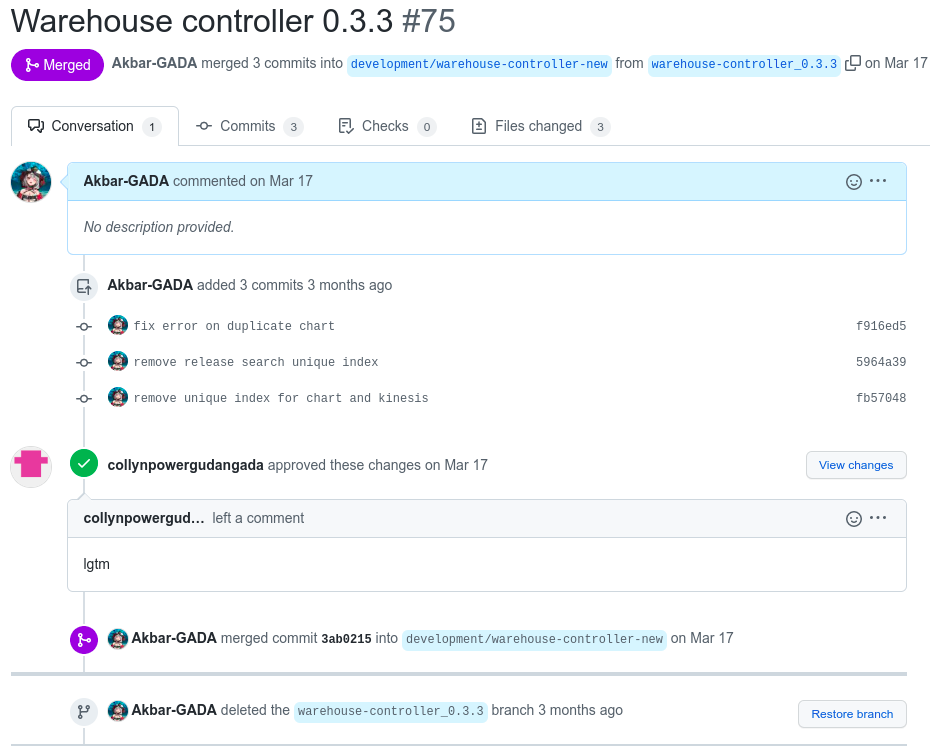
\includegraphics[width=1\textwidth]{pics/wc-lgtm.png}
	\caption{Pemilik repositori memberikan lampu hijau untuk melakukan \textit{merge} ke repositori Data Warehouse GudangAda}
	\label{fig:wcLGTM}
\end{figure}

\subsection{Membuat dan Mengirimkan Docker \textit{Image} ke Repositori GudangAda}
\label{sec:uploadDocker}

Setelah aplikasi disetujui oleh pemilik repositori, aplikasi dapat di kemas ke dalam sebuah \textit{image} dan dikirimkan ke repositori GudangAda. Pembuatan \textit{image} dilakukan dengan menjalankan perintah \code{docker build -t IMAGE\_NAME:TAG .} pada direktori aplikasi. Hasil dari perintah tersebut dapat dilihat pada gambar \ref{fig:dockerBuild}

\begin{figure}
	\centering
	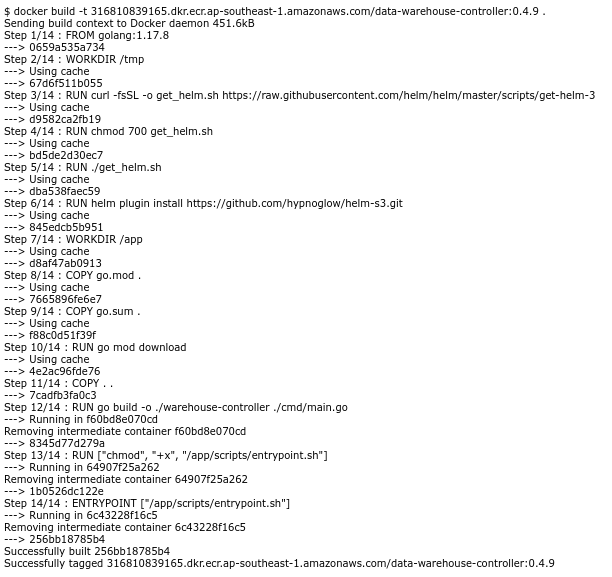
\includegraphics[width=1\textwidth]{pics/image-build.png}
	\caption{Membuat Docker \textit{image}}
	\label{fig:dockerBuild}
\end{figure}

Setelah \textit{image} aplikasi berhasil dibuat, \textit{image} tersebut harus dikirimkan ke repositori GudangAda. Hal ini dilakukan agar Terraform dapat memakai \textit{image} yang telah dibuat. Pengiriman \textit{image} dilakukan dengan perintah \code{docker push IMAGE\_NAME:TAG}. Hasil dari perintah tersebut dapat dilihat pada gambar \ref{fig:dockerPush}

\begin{figure}
	\centering
	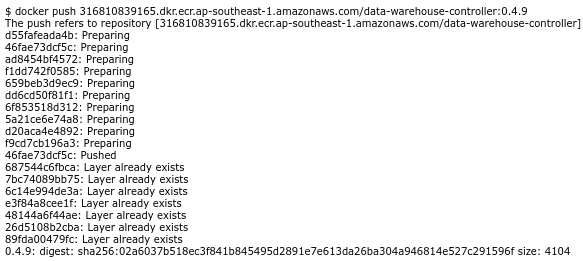
\includegraphics[width=1\textwidth]{pics/image-push.png}
	\caption{Mengirimkan Docker \textit{image} ke repositori GudangAda}
	\label{fig:dockerPush}
\end{figure}

\subsection{Data Helm Chart}
\label{sec:mergeHelmChart}

GudangAda menggunakan Amazon S3 sebagai repositori Helm Chart. Repositori tersebut tersinkronsasi dengan repositori GitHub \code{data-helm-chart}. Semua kode yang berada pada branch master akan ditambahkan ke Amazon S3. Oleh karena itu, proses untuk menambahkan Helm Chart ke repositori Amazon S3 adalah membuat \textit{merge request} untuk diperiksa oleh pemilik repositori. Setelah pemilik repositori menyetujui Helm Chart yang ditulis, Helm Chart tersebut dapat digabungkan dengan Helm Chart lain pada repositori GitHub. 

\begin{figure}
	\centering
	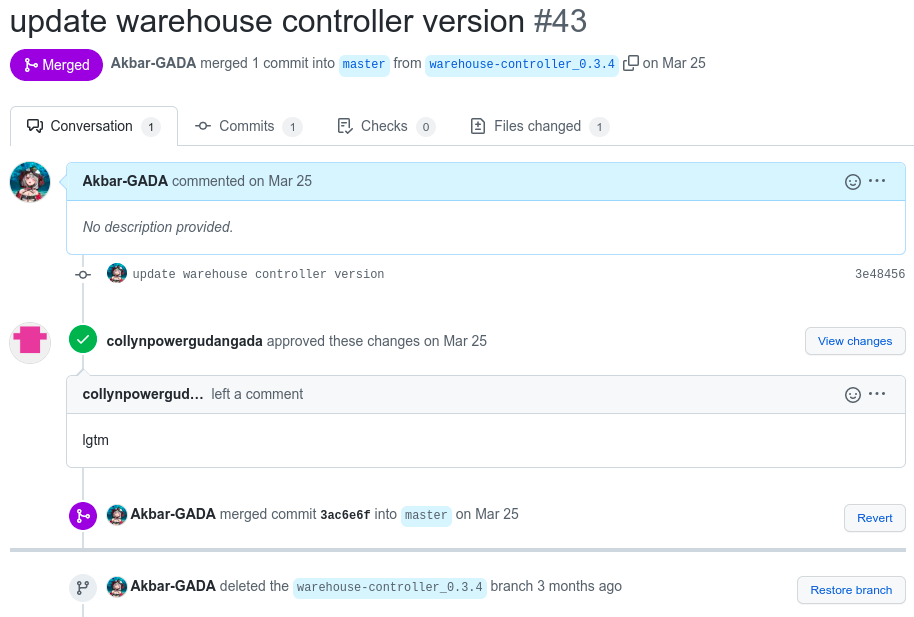
\includegraphics[width=0.75\textwidth]{pics/chart-lgtm.png}
	\caption{Pemilik repositori memberikan lampu hijau untuk melakukan \textit{merge} ke repositori Data Helm Chart pada GitHub GudangAda}
	\label{fig:wcLGTMTF}
\end{figure}

\subsection{Data IAAC}
\label{sec:mergeTerraform}
Proses \textit{deployment} menggunakan Terraform dilakukan dengan membuat \textit{request merge} ke \textit{repository} data IAAC. Setelah pemilik repositori melakukan \textit{review} terhadap perubahan yang akan dilakukan. Proses \textit{deployment} dapat dimulai.

\begin{figure}
	\centering
	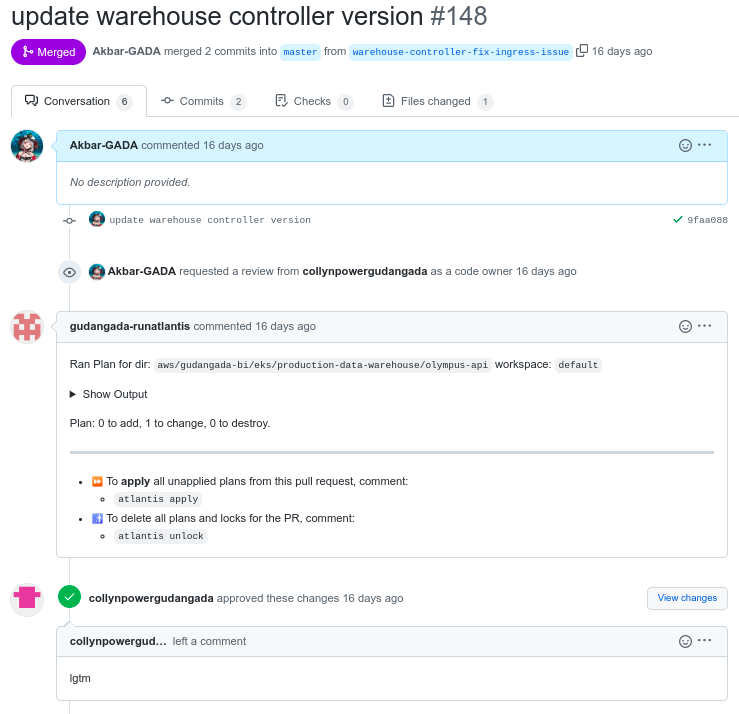
\includegraphics[width=0.75\textwidth]{pics/github-lgtm.png}
	\caption{Pemilik repositori memberikan lampu hijau untuk memulai proses deployment}
	\label{fig:githubLGTM}
\end{figure}

Proses \textit{deployment} dilakukan dengan melakukan \code{atlantis plan}, perintah ini bertujuan untuk menghitung semua kebutuhan \textit{deployment}, \code{atlantis plan} dilakukan secara otomatis saat \textit{merge request} dibuat. Setelah perintah \code{atlantis plan} selesai, akan dikirimkan perintah \code{atlantis apply} untuk menjalankan semua kebutuhan \textit{deployment} yang didapat dari \code{atlantis plan}. Setelah perintah \code{atlantis apply} selesai, kode sudah berhasil di deploy dan kode dapat di \textit{merge} ke repositori GudangAda.

\begin{figure}
	\centering
	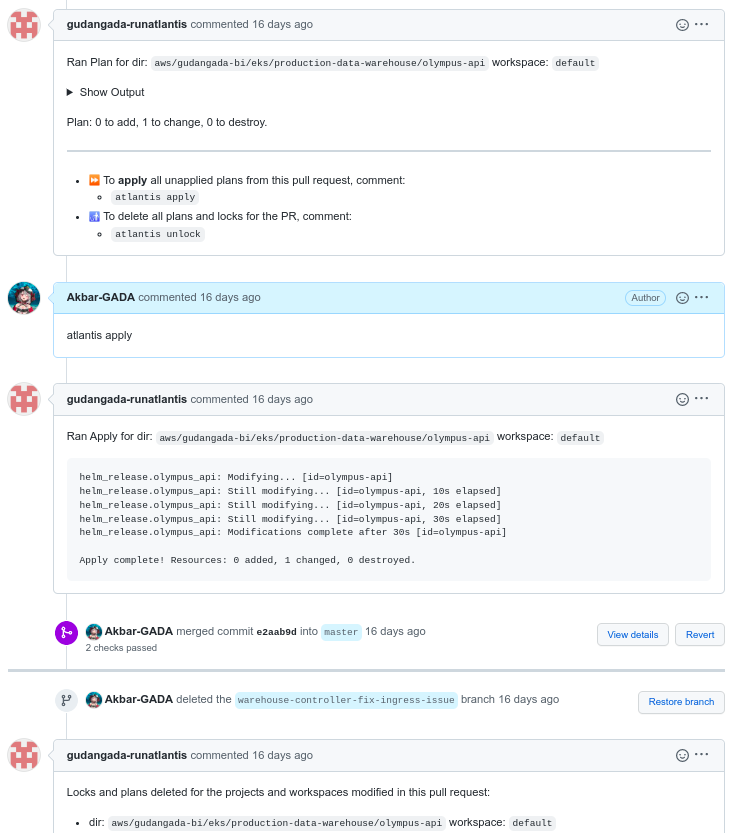
\includegraphics[width=0.75\textwidth]{pics/github-merge.png}
	\caption{Proses deployment menggunakan Terraform}
	\label{fig:githubMerge}
\end{figure}
\clearchapter
%-----------------------------------------------------------------------------%
\chapter{\babLima}
\label{bab:5}
%-----------------------------------------------------------------------------%
Bab ini akan memaparkan detail terkait uji penggunaan dalam upaya melakukan
verifikasi serta pengujian terhadap implementasi yang telah dilakukan berdasarkan
berbagai proses analisis dan perancangan.


\section{Pengujian melakukan \textit{deployment} Helm chart}
Pengujian dilakukan dengan tujuan untuk memastikan bahwa fitur \textit{deployment} Helm Chart dapat digunakan dan dapat berjalan sesuai dengan ekspektasi yang telah didefinisikan.
\subsection{Prekondisi}
Prekondisi yang diberikan sebelum proses pengujian dilaksanakan adalah:
\begin{itemize}
    \item Terdapat spesifikasi Helm Chart yang belum di \textit{deploy}.
\end{itemize}
\subsection{Ekspektasi}
Ekspektasi yang diberikan terhadap proses pengujian adalah:
\begin{itemize}
    \item Pengguna dapat mengirimkan perintah untuk melakukan \textit{deployment} Helm Chart.
    \item Aplikasi akan mengirimkan respons sukses.
    \item Spesifikasi Helm Chart yang diinginkan telah di \textit{deploy}.
\end{itemize}
\subsection{Hasil}
Hasil pengujian terhadap ekspektasi yang diberikan dan prekondisi yang telah ditentukan adalah:
\begin{enumerate}
    \item Dapat dilihat bahwa tidak ada pod yang sedang berjalan pada \textit{environment} Kubernetes.
    \begin{figure}
    	\centering
    	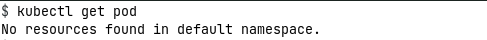
\includegraphics[width=0.8\textwidth]{pics/5.1.GetPod.png}
    	\caption{Kondisi awal Kubernetes}
    	\label{fig:getPod}
    \end{figure}
    \item Perintah untuk membuat deployment Helm chart baru dikirimkan melalui curl dan aplikasi memberikan respons sukses.
    \begin{figure}
    	\centering
    	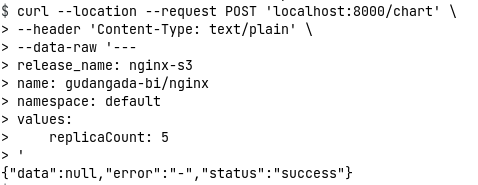
\includegraphics[width=0.8\textwidth]{pics/5.1.Curl.png}
    	\caption{Perintah \textit{deploy} Helm}
    	\label{fig:deployHelm}
    \end{figure}    
    \item Hasil akhir dapat dilihat dengan menjalankan perintah 'kubectl get pod'.
    \begin{figure}
    	\centering
    	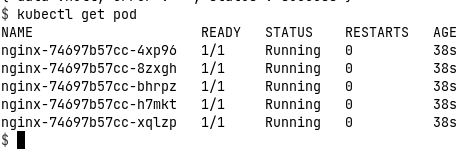
\includegraphics[width=0.8\textwidth]{pics/5.1.FinalGetPod.png}
    	\caption{Kondisi Kubernetes setelah perintah \textit{deployment}}
    	\label{fig:getPodFinal}
    \end{figure}
\end{enumerate}


\section{Pengujian melakukan \textit{deployment} Helm Chart pada \textit{namespace} yang berbeda-beda}
Pengujian dilakukan dengan tujuan untuk memastikan bahwa \textit{deployment} pada banyak \textit{namespace} dapat digunakan dan dapat berjalan sesuai dengan ekspektasi yang telah didefinisikan.

\subsection{Prekondisi}
Prekondisi yang diberikan sebelum proses pengujian dilaksanakan adalah:
\begin{itemize}
    \item Aplikasi telah dikonfigurasikan untuk dapat melayani \textit{namespace} yang dipakai untuk \textit{deployment}.
    \item Target \textit{namespace} yang akan dipakai untuk pengujian kali ini adalah test, test-2, dan test-3
    \item Terdapat beberapa spesifikasi Helm Chart yang belum di \textit{deploy}, masing-masing akan di \textit{deploy} pada \textit{namespace} yang berbeda.
\end{itemize}
\subsection{Ekspektasi}
Ekspektasi yang diberikan terhadap proses pengujian adalah:
\begin{itemize}
    \item Pengguna dapat mengirimkan perintah untuk melakukan \textit{deployment} Helm Chart.
    \item Aplikasi akan mengirimkan respons sukses.
    \item Spesifikasi Helm Chart yang diinginkan telah di \textit{deploy} dan sesuai dengan \textit{namespace} yang dispesifikasikan.
\end{itemize}
\subsection{Hasil}
Hasil pengujian terhadap ekspektasi yang diberikan dan prekondisi yang telah ditentukan adalah:
\begin{enumerate}
    \item Perintah untuk membuat \textit{deployment} Helm chart baru dikirimkan melalui curl untuk masing-masing \textit{namespace} dan aplikasi memberikan respons sukses.
    \begin{figure}
    	\centering
    	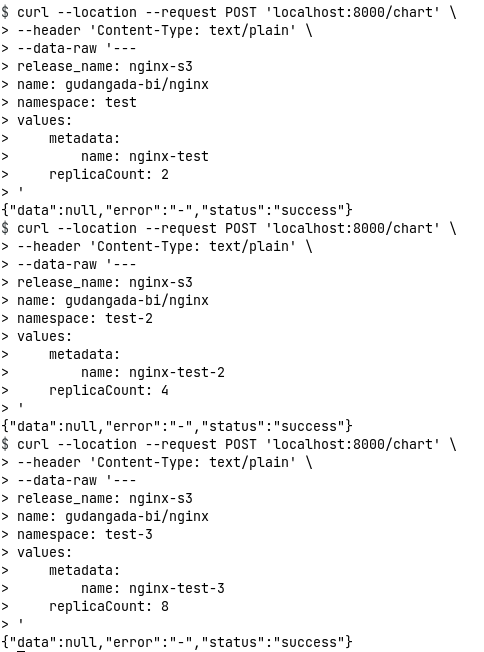
\includegraphics[width=0.5\textwidth]{pics/5.2.curl.png}
    	\caption{Perintah \textit{deployment} Helm pada masing-masing \textit{namespace}}
    	\label{fig:curlNamespace}
    \end{figure}
    \item Hasil akhir dapat dilihat dengan menjalankan perintah 'kubectl get pod -n \{namespace\}'.
    \begin{figure}
    	\centering
    	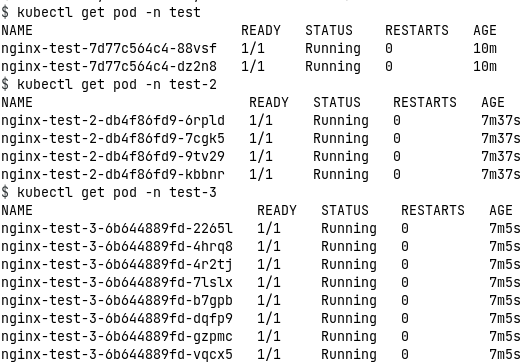
\includegraphics[width=0.8\textwidth]{pics/5.2.get-pod.png}
    	\caption{Kondisi Kubernetes setelah perintah \textit{deployment} pada masing-masing \textit{namespace}}
    	\label{fig:getPodFinalNamespace}
    \end{figure}
    
\end{enumerate}


\section{Pengujian melakukan \textit{deployment} AWS Kinesis}
Pengujian dilakukan dengan tujuan untuk memastikan bahwa fitur \textit{deployment} AWS Kinesis dapat digunakan dan dapat berjalan sesuai dengan ekspektasi yang telah didefinisikan.
\subsection{Prekondisi}
Prekondisi yang diberikan sebelum proses pengujian dilaksanakan adalah:
\begin{itemize}
    \item Terdapat spesifikasi AWS Kinesis yang belum di \textit{deploy}.
\end{itemize}
\subsection{Ekspektasi}
Ekspektasi yang diberikan terhadap proses pengujian adalah:
\begin{itemize}
    \item Pengguna dapat mengirimkan perintah untuk melakukan \textit{deployment} AWS Kinesis.
    \item Aplikasi akan mengirimkan respons sukses.
    \item Spesifikasi AWS Kinesis yang diinginkan telah di \textit{deploy}.
\end{itemize}
\subsection{Hasil}
Hasil pengujian terhadap ekspektasi yang diberikan dan prekondisi yang telah ditentukan adalah:
\begin{enumerate}
    \item Perintah untuk membuat AWS Kinesis baru dikirimkan melalui curl dan aplikasi memberikan respons sukses.
    \begin{figure}
    	\centering
    	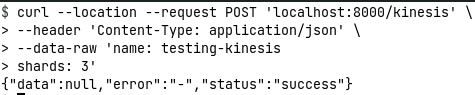
\includegraphics[width=1\textwidth]{pics/5.3.curl.png}
    	\caption{Perintah \textit{deployment} AWS Kinesis}
    	\label{fig:curlAwsKinesis}
    \end{figure}
    \item Hasil akhir\footnote{Karena pengujian AWS Kinesis dilakukan pada \textit{environment production}, maka terdapat \textit{instances} lain yang namanya di awali dengan 'production.****'. Untuk alasan keamanan, nama lengkap \textit{instance} AWS Kinesis lain akan disembunyikan.} dapat dilihat dengan menjalankan perintah 'aws kinesis list-streams'. 
    
    \begin{figure}
    	\centering
    	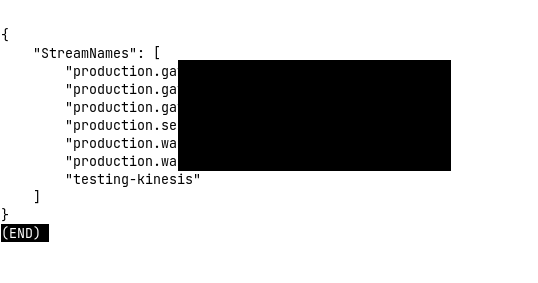
\includegraphics[width=1\textwidth]{pics/5.3.listStreams.png}
    	\caption{Hasil dari \textit{deployment} AWS Kinesis}
    	\label{fig:awsKinesis}
    \end{figure}
\end{enumerate}

\section{Pengujian melakukan \textit{templating} untuk \textit{deployment} Helm Chart dan Kinesis}
\label{sec:templateTest}
Pengujian dilakukan dengan tujuan untuk memastikan bahwa \textit{templating} dapat digunakan dan dapat berjalan sesuai dengan ekspektasi yang telah didefinisikan.
\subsection{Prekondisi}
Prekondisi yang diberikan sebelum proses pengujian dilaksanakan adalah:
\begin{itemize}
    \item Terdapat spesifikasi \textit{template} yang berisi spesifikasi Helm Chart dan AWS Kinesis yang belum di daftarkan.
    \item Terdapat spesifikasi yang dapat diisikan ke dalam \textit{template} untuk di \textit{deploy}.
\end{itemize}
\subsection{Ekspektasi}
Ekspektasi yang diberikan terhadap proses pengujian adalah:
\begin{itemize}
    \item Pengguna dapat mendaftarkan \textit{template} ke aplikasi yang dikerjakan.
    \item Pengguna dapat mengirimkan perintah untuk melakukan \textit{deployment} sesuai dengan spesifikasi yang dimiliki.
    \item Aplikasi akan mengirimkan respons sukses.
    \item Spesifikasi yang telah dikirimkan berhasil di \textit{deploy}.
\end{itemize}
\subsection{Hasil}
Hasil pengujian terhadap ekspektasi yang diberikan dan prekondisi yang telah ditentukan adalah:
\begin{enumerate}
    \item Perintah untuk membuat definisi \textit{template} dilakukan melalui curl.
    \begin{figure}
    	\centering
    	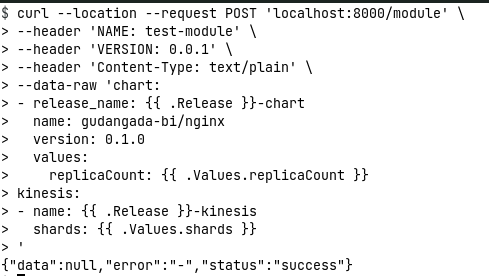
\includegraphics[width=0.8\textwidth]{pics/5.4.curlInitModule.png}
    	\caption{Inisiasi \textit{template}}
    	\label{fig:initTemplate}
    \end{figure}
    \item Perintah untuk membuat \textit{deployment} berdasarkan \textit{template} yang telah dibuat dilakukan melalui curl.
    \begin{figure}
    	\centering
    	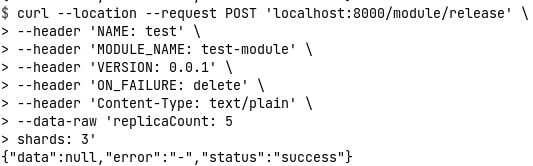
\includegraphics[width=0.8\textwidth]{pics/5.4.curlResult.png}
    	\caption{Penggunaan template}
    	\label{fig:templateUsage}
    \end{figure}
    \item Hasil akhir dapat dilihat dengan menjalankan perintah 'kubectl get pod' dan 'aws kinesis list-streams'
    \begin{figure}
    	\centering
    	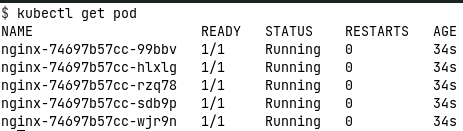
\includegraphics[width=0.8\textwidth]{pics/5.4.getPod.png}
    	\caption{Hasil kubectl get pod}
    	\label{fig:getPodTemplate}
    \end{figure}
    \begin{figure}
    	\centering
    	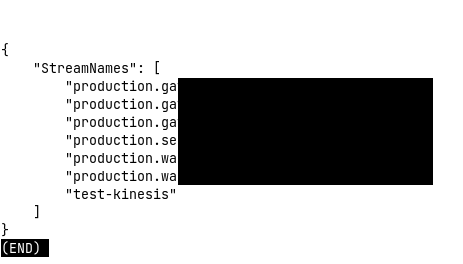
\includegraphics[width=0.8\textwidth]{pics/5.4.listStreams.png}
    	\caption{Hasil aws kinesis list-streams}
    	\label{fig:listStream}
    \end{figure}
\end{enumerate}


\section{Pengujian melakukan pengambilan variabel rahasia}
Pengujian dilakukan dengan tujuan untuk memastikan bahwa Vault dapat digunakan dan dapat berjalan sesuai dengan ekspektasi yang telah didefinisikan.
\subsection{Prekondisi}
Prekondisi yang diberikan sebelum proses pengujian dilaksanakan adalah:
\begin{itemize}
    \item Terdapat spesifikasi \textit{template} yang berisi spesifikasi Helm Chart yang memiliki variabel rahasia.
    \item Terdapat variabel rahasia yang dikelola oleh Vault yang dapat diakses oleh aplikasi.
    \begin{figure}
    	\centering
    	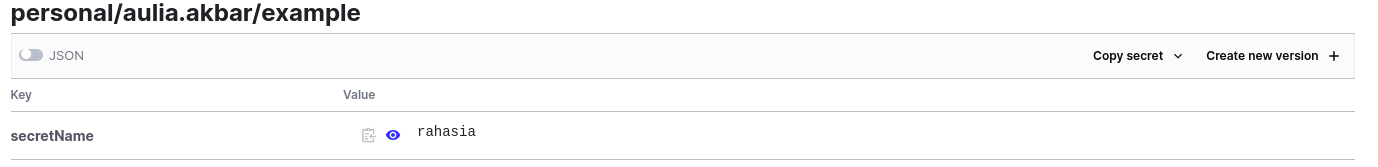
\includegraphics[width=0.8\textwidth]{pics/5.5.vault.png}
    	\caption{Variabel rahasia pada Vault}
    	\label{fig:vault}
    \end{figure}
\end{itemize}
\subsection{Ekspektasi}
Ekspektasi yang diberikan terhadap proses pengujian adalah:
\begin{itemize}
    \item Pengguna dapat mendaftarkan \textit{template} ke aplikasi yang dikerjakan.
    \item Pengguna dapat mengirimkan perintah untuk melakukan \textit{deployment} sesuai dengan spesifikasi yang dimiliki.
    \item Variabel rahasia berhasil dimasukkan ke dalam spesifikasi final aplikasi yang akan di \textit{deploy}.
    \item Aplikasi akan mengirimkan respons sukses.
    \item Spesifikasi yang telah dikirimkan berhasil di \textit{deploy}.
\end{itemize}
\subsection{Hasil}
Hasil pengujian terhadap ekspektasi yang diberikan dan prekondisi yang telah ditentukan adalah:
\begin{enumerate}
    \item Perintah untuk membuat definisi \textit{template} yang mengandung variabel rahasia dilakukan melalui curl.
    \begin{figure}
    	\centering
    	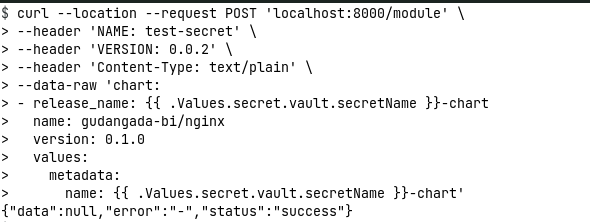
\includegraphics[width=0.8\textwidth]{pics/5.5.initTemplate.png}
    	\caption{Inisiasi \textit{template} yang mengandung variabel rahasia}
    	\label{fig:initTemplateSecret}
    \end{figure}
    \item Perintah untuk membuat \textit{deployment} berdasarkan \textit{template} yang mengandung variabel rahasia dilakukan melalui curl.
    \begin{figure}
    	\centering
    	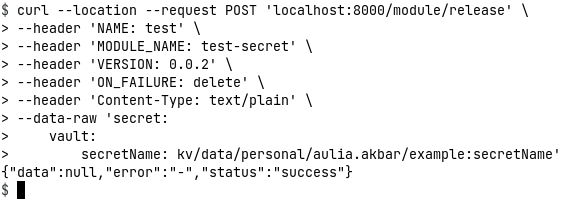
\includegraphics[width=0.8\textwidth]{pics/5.5.useTemplate.png}
    	\caption{Penggunaan \textit{template} yang mengandung variabel rahasia}
    	\label{fig:useTemplateSecret}
    \end{figure}
    \item Terlihat bahwa variabel rahasia dapat
    dilihat\footnote{Penulis membuat agar variabel rahasia dapat terlihat(dibuat sebagai nama pod) agar mudah untuk melakukan verifikasi, pada penggunaan di dunia nyata variabel biasanya tidak diperlihatkan} sebagai nama pod pada perintah 'kubectl get pod'.
    \begin{figure}
    	\centering
    	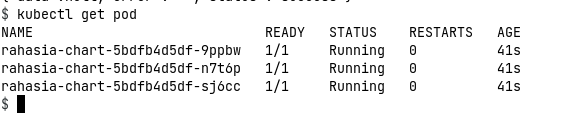
\includegraphics[width=0.8\textwidth]{pics/5.5.getPod.png}
    	\caption{Hasil kubectl get pod pada \textit{template} yang mengandung variabel rahasia}
    	\label{fig:getPodSecret}
    \end{figure}
\end{enumerate}


\section{Pengujian melakukan perubahan pada \textit{deployment} yang telah dibuat}
Pengujian dilakukan dengan tujuan untuk memastikan bahwa \textit{deployment} yang telah dilakukan dapat diubah sesuai dengan ekspektasi yang telah didefinisikan.
\subsection{Prekondisi}
Prekondisi yang diberikan sebelum proses pengujian dilaksanakan adalah:
\begin{itemize}
    \item Akan digunakan \textit{deployment} dari percobaan \ref{sec:templateTest} untuk di ubah detail spesifikasinya.
\end{itemize}
\subsection{Ekspektasi}
Ekspektasi yang diberikan terhadap proses pengujian adalah:
\begin{itemize}
    \item Pengguna dapat mengirimkan perintah untuk mengubah spesifikasi dari Helm Chart yang telah di \textit{deploy}.
    \item Aplikasi akan mengirimkan respons sukses.
    \item Helm Chart yang sebelumnya telah di \textit{deploy} berhasil diganti spesifikasinya.
\end{itemize}
\subsection{Hasil}
Hasil pengujian terhadap ekspektasi yang diberikan dan prekondisi yang telah ditentukan adalah:
\begin{enumerate}
    \item Perintah untuk mengubah \textit{deployment} yang telah dibuat dilakukan melalui curl.
    \begin{figure}
    	\centering
    	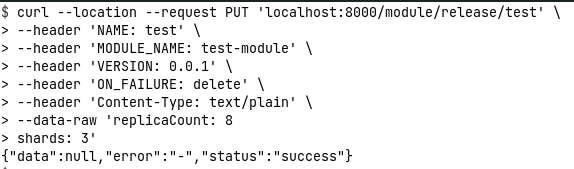
\includegraphics[width=0.8\textwidth]{pics/5.6.curl.png}
    	\caption{Perintah untuk mengubah \textit{deployment}}
    	\label{fig:putDeployment}
    \end{figure}
    \item Dapat dilihat bahwa jumlah \textit{instance pod} bertambah dari 5 menjadi 8.
    \begin{figure}
    	\centering
    	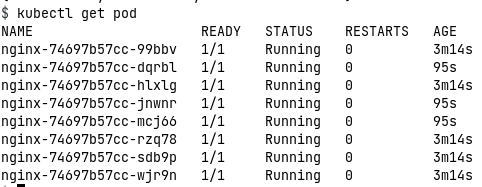
\includegraphics[width=0.8\textwidth]{pics/5.6.getPod.png}
    	\caption{Hasil dari kubectl get pod}
    	\label{fig:putKubectlGetPod}
    \end{figure}
\end{enumerate}


\section{Pengujian melihat detail dari deployment yang telah dibuat}
Pengujian dilakukan dengan tujuan untuk memastikan bahwa fitur melihat detail dari deployment yang telah dibuat dapat digunakan dan dapat berjalan sesuai dengan ekspektasi yang telah didefinisikan.
\subsection{Prekondisi}
Prekondisi yang diberikan sebelum proses pengujian dilaksanakan adalah:
\begin{itemize}
    \item Akan digunakan \textit{deployment} dari percobaan \ref{sec:templateTest} untuk di lihat detail spesifikasinya.
\end{itemize}
\subsection{Ekspektasi}
Ekspektasi yang diberikan terhadap proses pengujian adalah:
\begin{itemize}
    \item Pengguna dapat mengirimkan perintah untuk melihat spesifikasi dari Helm Chart yang telah di \textit{deploy}.
    \item Aplikasi akan mengirimkan respons sukses.
    \item Respons berisi detail dari aplikasi yang telah di \textit{deploy}.
\end{itemize}
\subsection{Hasil}
Hasil pengujian terhadap ekspektasi yang diberikan dan prekondisi yang telah ditentukan adalah:
\begin{enumerate}
    \item Perintah untuk melihat detail dari \textit{deployment} yang telah dibuat dilakukan melalui curl.
    \begin{figure}
    	\centering
    	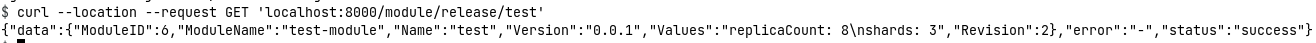
\includegraphics[width=1\textwidth]{pics/5.7.getDeployment.png}
    	\caption{Perintah untuk melihat detail \textit{deployment}}
    	\label{fig:getDeployment}
    \end{figure}
\end{enumerate}


\section{Pengujian menghapus \textit{deployment} yang telah dibuat}
Pengujian dilakukan dengan tujuan untuk memastikan bahwa \textit{deployment} yang telah dibuat dapat dihapus sesuai dengan ekspektasi yang telah didefinisikan.
\subsection{Prekondisi}
Prekondisi yang diberikan sebelum proses pengujian dilaksanakan adalah:
\begin{itemize}
    \item Akan digunakan \textit{deployment} dari percobaan \ref{sec:templateTest} untuk di hapus.
\end{itemize}
\subsection{Ekspektasi}
Ekspektasi yang diberikan terhadap proses pengujian adalah:
\begin{itemize}
    \item Pengguna dapat mengirimkan perintah untuk menghapus \textit{deployment} Helm Chart.
    \item Aplikasi akan mengirimkan respons sukses.
    \item Kondisi \textit{deployment} Helm Chart yang ada telah dihapus.
\end{itemize}
\subsection{Hasil}
Hasil pengujian terhadap ekspektasi yang diberikan dan prekondisi yang telah ditentukan adalah:
\begin{enumerate}
    \item Perintah untuk menghapus \textit{deployment} yang telah dibuat dilakukan melalui curl.
    \begin{figure}
    	\centering
    	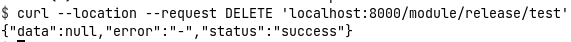
\includegraphics[width=1\textwidth]{pics/5.8.curl.png}
    	\caption{Perintah untuk menghapus \textit{deployment}}
    	\label{fig:deleteDeployment}
    \end{figure}
    \item Terlihat bahwa pada 'kubectl get pod' dan 'aws kinesis list-streams' sudah tidak ada lagi \textit{instance} dari percobaan \ref{sec:templateTest}.
    \begin{figure}
    	\centering
    	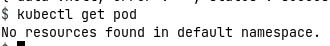
\includegraphics[width=0.8\textwidth]{pics/5.8.getPod.png}
    	\caption{Hasil kubectl get pod}
    	\label{fig:getPodDeleted}
    \end{figure}
    \begin{figure}
    	\centering
    	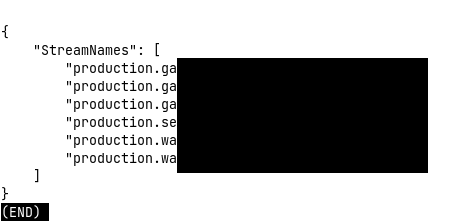
\includegraphics[width=0.8\textwidth]{pics/5.8.listStreams.png}
    	\caption{Hasil aws kinesis list-streams}
    	\label{fig:listStreamDeleted}
    \end{figure}
    
\end{enumerate}


\section{Pengujian mencoba menghapus \textit{deployment} yang tidak dikendalikan oleh aplikasi}
Pengujian dilakukan dengan tujuan untuk memastikan bahwa pembatasan kontrol aplikasi berjalan sesuai dengan ekspektasi yang telah didefinisikan.
\subsection{Prekondisi}
Prekondisi yang diberikan sebelum proses pengujian dilaksanakan adalah:
\begin{itemize}
    \item Terdapat \textit{deployment} Helm Chart yang tidak diatur oleh aplikasi yang telah dikerjakan.
    \begin{figure}
    	\centering
    	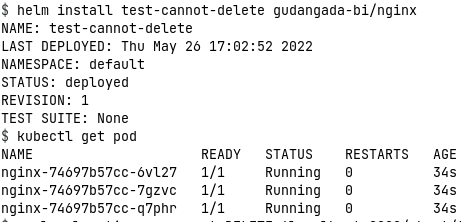
\includegraphics[width=0.8\textwidth]{pics/5.9.chartDeploymentAndGetPod.png}
    	\caption{\textit{Deployment} Helm Chart melalui Helm CLI}
    	\label{fig:helmChartUsingCLI}
    \end{figure}
\end{itemize}
\subsection{Ekspektasi}
Ekspektasi yang diberikan terhadap proses pengujian adalah:
\begin{itemize}
    \item Pengguna dapat mengirimkan perintah untuk menghapus \textit{deployment} Helm Chart.
    \item Aplikasi akan mengirimkan respons \textit{error}.
    \item Kondisi \textit{deployment} Helm Chart yang ada tidak berubah.
\end{itemize}
\subsection{Hasil}
Hasil pengujian terhadap ekspektasi yang diberikan dan prekondisi yang telah ditentukan adalah:
\begin{enumerate}
    \item Perintah untuk menghapus \textit{deployment} tidak dikontrol oleh aplikasi dilakukan melalui curl, namun terlihat bahwa perintah tersebut gagal.
    \begin{figure}
    	\centering
    	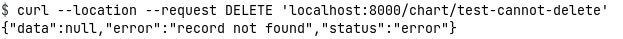
\includegraphics[width=1\textwidth]{pics/5.9.curl.png}
    	\caption{Perintah untuk menghapus \textit{deployment} yang tidak dikelola aplikasi}
    	\label{fig:deleteDeploymentFail}
    \end{figure}
    \item Terlihat bahwa pada 'kubectl get pod' tidak ada perubahan dari jumlah pod yang ada.
    \begin{figure}
    	\centering
    	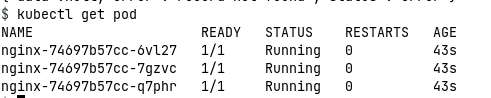
\includegraphics[width=0.8\textwidth]{pics/5.9.getPod.png}
    	\caption{Hasil kubectl get pod setelah operasi hapus gagal}
    	\label{fig:getPodFail}
    \end{figure}
\end{enumerate}
\clearchapter
%---------------------------------------------------------------
\chapter{\kesimpulan}
\label{bab:6}
%---------------------------------------------------------------
Pada bab ini, akan dipaparkan kesimpulan penelitian dan saran untuk penelitian berikut-nya.


%---------------------------------------------------------------
\section{Kesimpulan}
\label{sec:kesimpulan}
%---------------------------------------------------------------
Berikut ini adalah kesimpulan terkait pekerjaan yang dilakukan dalam penelitian ini:
\begin{enumerate}
	\item \bo{Integrasi Helm} \\
	Proses \textit{deployment} helm dapat diintegrasikan dengan aplikasi yang bekerja melalui \textit{HTTP request} dengan mengimplementasikan aplikasi yang memakai Helm \textit{API}. Aplikasi tersebut akan diimplementasikan dengan bahasa pemrograman Golang. Aplikasi akan menerima \textit{HTTP request} dari pengguna, setelah itu akan melakukan \textit{parsing data}, melakukan \textit{preprocessing}, dan terakhir akan meneruskannya ke API milik Helm untuk di \textit{deploy}.
	\item \bo{Integrasi Vault dan Amazon Kinesis} \\
	Dari rancangan pada bagian \ref{sec:vaultEngine} untuk Vault dan bagian \ref{sec:perancanganArsitektur} untuk Amazon Kinesis, serta implementasi pada bagian \ref{sec:initVault} dan \ref{sec:initKinesis}, dan telah diujikan fitur-fiturnya pada bab \ref{bab:5}. Dapat disimpulkan bahwa Vault dan Amazon Kinesis dapat diintegrasikan dengan aplikasi yang dikerjakan untuk membantu proses \textit{deployment}.
	\item \bo{Analisis terhadap Terraform} \\
    Pada bagian \ref{sec:terraform} dibuat spesifikasi pada Terraform dan dilakukan \textit{deployment} pada bagian \ref{sec:mergeTerraform}, proses tersebut membutuhkan pengguna untuk mendefinisikan 4 berkas untuk membuat satu buah \textit{deployment}. Sedangkan pada bagian \ref{sec:templateTest} hanya dibutuhkan 1 \textit{request} untuk membuat \textit{template} dan 1 \textit{request} untuk melakukan \textit{deployment}. Jika terdapat 5 \textit{deployment} dengan spesifikasi yang mirip, Terraform membutuhkan pengguna untuk menspesifikasikan 20 berkas, namun aplikasi yang dikembangkan hanya membutuhkan 6 \textit{HTTP request} untuk melakukan \textit{deployment} yang sama. Sehingga dapat disimpulkan bahwa penggunaan \textit{templating} pada aplikasi dapat mensimplifikasi proses \textit{deployment} dibandingkan dengan Terraform.
\end{enumerate}

%---------------------------------------------------------------
\section{Saran}
\label{sec:saran}
%---------------------------------------------------------------
Berdasarkan hasil penelitian ini, berikut ini adalah saran untuk pengembangan penelitian berikutnya:
\begin{enumerate}
	\item Kontrol aplikasi hanya dapat dilakukan pada Kubernetes Cluster yang sama pada tempat aplikasi tersebut berjalan. Hal ini dapat memaksa untuk dibuatnya banyak \textit{instance} aplikasi pada tiap Kubernetes Cluster. Kontrol antar cluster diharapkan untuk dapat diimplementasi untuk dapat menangani hal tersebut.
	\item Belum adanya sistem autentikasi dalam penggunaan aplikasi. Hal ini dapat menyebabkan siapapun yang dapat melakukan \textit{HTTP Request} ke aplikasi memiliki akses penuh kedalam aplikasi dan semua deployment yang dikontrol. Sistem autentikasi diharapkan untuk dapat diimplementasi untuk dapat menangani hal tersebut.
	\item Belum adanya \textit{Graphical User Interface}(GUI). Pengguna harus membuat HTTP Request melalui aplikasi pihak ketiga seperti CURL maupun Postman untuk dapat mengakses aplikasi. \textit{Website Front-end }diharapkan untuk dapat diimplementasi untuk dapat menangani hal tersebut.
\end{enumerate}

\clearchapter

%
% Daftar Pustaka
\CAPinToC % All entries in ToC will be CAPITALIZED from here on
%
% Daftar Pustaka
%

%
% Tambahkan pustaka yang digunakan setelah perintah berikut.
%
\renewcommand{\bibname}{Daftar Referensi}
\renewcommand{\refname}{Daftar Referensi}
\phantomsection %hack to add clickable section for pustaka
\bibliographystyle{apacite}
\bibliography{references}

\clearchapter
\noCAPinToC % Revert to original \addcontentsline formatting

%
% Lampiran
%
\begin{appendix}
	\newcounter{pagetemp}
	\setcounter{pagetemp}{\thepage}
	%
% @author  Andreas Febrian
% @version 1.00
%
% Hanya sebuah pembatas bertuliskan LAMPIRAN ditengah halaman.
%

\begin{titlepage}
\centering
\vspace*{6cm}
\noindent \Huge{LAMPIRAN}
\end{titlepage}

	\clearchapter
	\setcounter{page}{\thepagetemp}
	\stepcounter{page}
	%-----------------------------------------------------------------------------%
\addappendix{Hasil Akhir Aplikasi}
\chapter*{Lampiran 1: Kode Hasil Akhir Aplikasi}
\label{appendix:hasilAplikasi}
%-----------------------------------------------------------------------------%
Semua kode aplikasi yang dikembangkan dapat diakses pada repositori:\\
\url{https://github.com/Xerdiosa/Skripsi-Helm-Controller-App}

%-----------------------------------------------------------------------------%
\addappendix{Helm Chart Aplikasi}
\chapter*{Lampiran 2: Helm Chart Aplikasi}
\label{appendix:helmChartAplikasi}
%-----------------------------------------------------------------------------%
Helm Chart yang dipakai untuk deployment aplikasi yang dikembangkan dapat diakses pada repositori:\\
\url{https://github.com/Xerdiosa/Skripsi-Helm-Controller-Chart}

%-----------------------------------------------------------------------------%
\addappendix{Konfigurasi Terraform Aplikasi}
\chapter*{Lampiran 3: Konfigurasi Terraform Aplikasi}
\label{appendix:terraformAplikasi}
%-----------------------------------------------------------------------------%
Helm Chart yang dipakai untuk deployment aplikasi yang dikembangkan dapat diakses pada repositori:\\
\url{https://github.com/Xerdiosa/Skripsi-Helm-Controller-Terraform}
\end{appendix}

\end{document}